% This is samplepaper.tex, a sample chapter demonstrating the
% LLNCS macro package for Springer Computer Science proceedings;
% Version 2.20 of 2017/10/04
%
\documentclass[runningheads]{llncs}
\usepackage{amsmath}
\usepackage{amssymb}
\usepackage{mathrsfs}
\usepackage{graphicx}
\usepackage{subfigure}
\usepackage{physics}
\usepackage{tikz} 
\usepackage{scalefnt}
\usepackage{qcircuit}
\usepackage{tabularx} 
\usepackage{float}
 

\usepackage[linesnumbered,ruled,lined]{algorithm2e}
% Used for displaying a sample figure. If possible, figure files should
% be included in EPS format.
%
% If you use the hyperref package, please uncomment the following line
% to display URLs in blue roman font according to Springer's eBook style:
% \renewcommand\UrlFont{\color{blue}\rmfamily}

\begin{document}
%
\title{Quantum Circuit Transformation Based on GraphQL and Tabu Search\thanks{Supported by organization x.}}
%
%\titlerunning{Abbreviated paper title}
% If the paper title is too long for the running head, you can set
% an abbreviated paper title here
%
\author{First Aaaaaaauthor\inst{1}\orcidID{0000-ereer1111-2222-3333} \and
Second Author\inst{2,3}\orcidID{1111-2222-3333-4444} \and
Third Author\inst{3}\orcidID{2222--3333-4444-5555}}
%
\authorrunning{F. Author et al.}
% First names are abbreviated in the running head.
% If there are more than two authors, 'et al.' is used.
%
\institute{Princeton University, Princeton NJ 08544, USA \and
Springer Heidelberg, Tiergartenstr. 17, 69121 Heidelberg, Germany
\email{lncs@springer.com}\\
\url{http://www.springer.com/gp/computer-science/lncs} \and
ABC Institute, Rupert-Karls-University Heidelberg, Heidelberg, Germany\\
\email{\{abc,lncs\}@uni-heidelberg.de}}
%
\maketitle              % typeset the header of the contribution
%
\begin{abstract}
	Since we are in the NISQ era, quantum systems are prone to interact with the surrounding environment 
	to generate noise, which can overwhelm the signal in the circuit. 
	One way to eliminate errors is to use quantum error correction. 
	Due to the limitation of circuit size, the computing power of NISQ technology is limited. 
	Quantum error correction brings heavy overhead in terms of the number of qubits and gates. 
	Therefore, it is difficult to achieve scale expansion using quantum error correction. 
	Currently, the quantum circuit we simulate ignores quantum noise. 
	In addition, the operation between qubits of NISQ devices is limited, 
	and only adjacent qubits can be operated. Therefore, a large number of modifications must 
	be made to the logic circuit to adapt to physical limitations. 
	It is vital to the success of quantum computing 
	how to find an automated method to effectively transform any input quantum circuit into a 
	quantum that satisfies the physical constraints imposed by the NISQ device 
	and has a small overhead in terms of number of auxiliary gates, circuit depth or errors circuit.
	This paper mainly summarizes the advantages and disadvantages of current quantum algorithms, and adjusts the life cycle of qubits through preprocessing of quantum circuits to increase the parallelism of quantum circuits.
	Then, the GraphQL combined subgraph isomorphism algorithm is used to generate high-quality initial mapping, and finally a circuit transformation algorithm based on Tabu Search is proposed to obtain a multi-objective circuit that satisfies the constraints of logic circuits and physical circuits.
	 For a benchmark composed of 159 circuits and IBM Q20,
	  compared with the initial mapping based on the $VF$ algorithm, 
	  our initial mapping has an average efficiency improvement of 22.26\%. 
	  Our algorithm only needs 461 seconds to run all, 
	  and other state-of-the-art algorithms are difficult to handle large circuits.
\keywords{Quantum circuit transformation  \and  Subgraph isomorphism \and Initial mapping \and Tabu Search}
\end{abstract}
\section{Introduction}
\label{Introduction}
From the discovery of quantum mechanics in the early 20th century to the present,
quantum technology has been applied in practice, but large quantum computers
have not yet been established, and most of the contributions of quantum 
information to computer science are still in the theoretical stage.
In March 2017, IBM developed the first 5-qubits backend named IBM QX2. 
In June, it launched the second 16-qubits backend IBM QX3.
It was launched in December. The revised versions of 5-qubits and 16-qubits 
are called IBM QX4 and IBM QX5 respectively.
IBM Q provides the public with free quantum computer resources on the cloud. 
If we want to use these quantum computer resources, 
we must map quantum circuits to a given physical architecture and 
satisfy physical constraints. This requires a set of highly efficient and 
automatic mapping procedures. Quantum circuit transformation is an important 
part of quantum circuit compilation. The main idea is to convert the input
logic circuit into a physical logic circuit and satisfy the constraints of
the physical circuit.

There are currently five main methods for solving qubit allocation. 
The first method is to use the unit matrix factorization algorithm to rearrange 
the quantum circuit from the beginning while retaining the function of the input 
circuit\cite{2019CNOT,2019Quantum}.
The second method is to convert the quantum circuit transformation problem into 
some existing problems, such as AI planning \cite{2017Temporal,2018Integer}, 
Integer Linear Programming (ILP)\cite{2019Almeida}, 
Satisfiable Modulus Theory (SMT) \cite{2019Murali}, 
or using the ready-made tools for these problems to find acceptable results.
But these methods may run for a long time and 
can only be applied to a small amount of qubit. 
And these tools cannot take advantage of some of the properties of quantum mapping.
The third method is to use precise methods to construct output quantum circuits. 
This method is only suitable for simple quantum structures and cannot be extended to 
complex quantum structures\cite{2018QubitSiraichi}.
The fourth method is to use the relevant conclusions of graph theory.
\cite{Shafaei2013} use the minimum linear arrangement problem in graph theory 
to model the problem of reducing the interaction distance.
It divides a given circuit into several sub-circuits, 
and then applies the minimum linear arrangement problem respectively, 
and turns non-adjacent gates in the sub-circuits into adjacent circuits 
by adding auxiliary gates.
Finally it uses the minimum linear permutation problem to find a permutation, 
and uses bubble sort to calculate the number of SWAP gates needed.
In \cite{Guerreschi2018} and 2019 Matsuo A \cite{Matsuo2019}, 
a two-step approach is proposed to reformulate the subtasks 
of gate scheduling as a graph problem.
According to the graph coloring problem and the maximum subgraph isomorphism,
the SWAP operations are added to minimize its overhead.
Both of them move a qubit from the initial position to 
the target position in the best possible path with minimal cost.
The former defines a priority to get the initial mapping, 
and the latter is purely to solve the problem of position movement. 
They all divide the SWAP of qubits into three categories. 
The first is a movement that is beneficial to both qubits; 
the second is a qubit is advantageous, 
and the other qubit is not mapped; 
the third is that one qubit is advantageous and 
one qubit is harmful. 
Then they calculate the scores from the initial position 
to the target position according to the type, and move.
The fifth is to use heuristic search \cite{Zulehner2017,Cowtan2019,Li2018,Xiangzhen2020,2018QubitSiraichi},
the circuit mapping process hopes to find a minimum number of SWAPs, 
but it takes exponential time, 
so heuristic search is used to control the evaluation function 
to obtain an acceptable solution.
\cite{Zulehner2017} divides a given circuit into multiple layers, 
which can be implemented in a $CNOT$ 
constraint compatible manner. Then, for each of these layers, 
a respectively compatible mapping is determined, 
which requires as few additional gates as possible. 
The main idea is to determine the cheapest path from the root node to the target node 
(the path with the lowest cost). Since the search space is usually exponential, 
complex mechanisms are used to keep the paths considered as few as possible.
\cite{Xiangzhen2020} designs a heuristic search algorithm with a novel selection mechanism, 
in which in each step of the search process, we do not choose the lowest cost operation to be applied, 
but looks forward one step, and then chooses the best continuous operation operation. 
In this way, the algorithm can effectively avoid local minimum. And a pruning mechanism is introduced 
to reduce the size of the search space and ensure that the program terminates in a reasonable time. 
The time complexity of this algorithm is $O(|V|^{4})$.
\cite{Li2018} Proposes a SWAP-based search scheme SABRE. 
Comparing with previous search algorithms based on exhaustive mapping, 
this search scheme achieves an exponential acceleration of search complexity 
with the results of previous schemes.
This fast search scheme ensures the scalability of SABRE to adapt to the large 
quantum equipment in the NISQ era.
By introducing the attenuation effect in the heuristic cost function, 
different hardware compatible circuits are generated by switching the number 
of gates in the circuit according to the circuit depth.
This makes SABRE suitable for NISQ devices with different characteristics and optimization goals.
The routing algorithm implemented in $t\ket{ket}$\cite{Cowtan2019} can ensure 
that any quantum circuit is compiled into any architecture.
The algorithm is divided into four stages: 
decomposing the input circuit into time steps, 
determining the initial position, 
routing across time steps, and finally cleaning up.
The heuristic method in $t\ket{ket}$ matches or is better than the results of 
other circuit mapping systems in terms of depth and total number of gates of 
the compiled circuit, and the running time is greatly reduced, allowing larger circuits to be routed.
2019 Tannu \cite{Tannu2019} proposed a Variation-aware Qubit Movement strategy, 
which takes advantage of the change in error rate and a change-aware qubit allocation 
strategy by trying to select the route with the lowest probability of failure. 
This strategy allocates program qubits to physical Qubits to take advantage 
of SWAPs in the error rate, thereby minimizing the use of links with high error rates.

In general, it can be used as an initial search algorithm to generate the initial solution. 
\cite{Paler2018} uses a heuristic method to find the initial mapping, and uses IBM's compiler to benchmark. 
The preliminary results show that the cost can be reduced by up to 10\% only by placing qubits 
that are different from the default position (trivial placement) only in the actual circuit instance 
on the actual NISQ architecture. Recently, a novel reverse traversal technique is proposed in \cite{Li2018}, 
which selects the initial mapping method considering the whole circuit. 
In \cite{Xiangzhen2020}, an annealing algorithm is proposed to find favorable initial mapping. 
The heuristic initial mapping generated by the scheme is unstable 
and can not be used in business. In \cite{2020Qubit}, VF subgraph isomorphism algorithm is 
used to generate initial mapping. 
Compared with VF mapping, our algorithm 
based on GraphQL reduces 
the number of SWAP gates by 22.29\% and the depth by 11.17\%.


The biggest problem facing quantum information processing is the problem of quantum decoherence.
The entanglement of the quantum system with the surrounding environment and quantum measurement 
will cause the disappearance of quantum coherence.
Since it is now in the Noisyed Intermiat-Scale Quantum (NISQ) era, there are only dozens of qubits, 
and it is unrealistic to realize quantum error correction\cite{2018QuantumPreskill}.
Quantum physical circuits are also limited. It is basically impossible to directly map logical circuit
to physical architecture graph, and quantum gate operations can only be performed between adjacent qubits, 
so it is necessary to convert the circuit by adding auxiliary gates are used to satisfy logical and physical 
constraints, and this process may introduce a lot of errors, 
which brings a huge challenge to the program compilation, because noise will have a greater impact on the 
final circuit and may make the result meaningless.

The main contributions of this paper are as follows.
	\begin{enumerate}
		\item This paper summarizes the current status, problems, and breakthrough directions 
		of the current quantum mapping work, and points out their advantages and disadvantages 
		to existing solutions. On this basis, this paper proposes a  
		combinated subgraph isomorphism initial mapping and Tabu Search heuristic SWAP search scheme GQLTS.
		\item Considering that the quantum coherence time is very short, 
		the longest coherence time of a superconducting quantum chip is still within 10us-100us, 
		the time of a single quantum gate is about 20ns, 
		the time of a 2-qubits gate is about 40ns, 
		and the time of measurement operation is about 300ns-1us.
		In order to ensure that the quantum operation is completed in the coherent time,
		we preprocess the quantum circuit to increase the parallelism of the quantum and 
		relatively reduce the depth of the output circuit.
		\item It has been proved that the initial mapping has a great influence on the quantum
		 circuit mapping, so we tried a variety of schemes, 
		 hoping to output the quantum circuit with the fewest auxiliary gates. 
		 In the end, we choose to use combined subgraph isomorphism to obtain 
		 a partial initial mapping set of qubits, 
		 and then use the vertex completion algorithm to map the unmapped qubits to the coupled graph. 
		 Compared with the VF2 subgraph isomorphism scheme, 
		combined subgraph isomorphism algorithm performs better.
		\item We propose a heuristic SWAP search scheme GQLTS based on Tabu Search, 
		which can handle large circuits in a short time at a low cost.
		Compared with the previous precise search and heuristic schemes,
		this scheme can complete the circuit transformation in a shorter time, 
		but GQLTS needs to be added compared to the wgtgraph algorithm Equal or more auxiliary gates.
		GQLTS can complete the search of the 159 circuits in this paper within a few minutes, 
		but the heuristic search takes a few days to get all the results, 
		and even the heuristic scheme may not get results when processing large circuits.
	\end{enumerate}
	The rest of this paper is arranged as follows. 
	Section~\ref{Background} introduces the background of quantum computing and quantum information.
	Section~\ref{Problem Analysis} analyzes the problems that need to be dealt with the transformation of quantum circuits.
	Section~\ref{Solution} introduces our algorithm in detail. 
	Section~\ref{Experiment} introduces the experiment and results, 
	and the last section summarizes the paper and discusses future research.

\section{Background}
\label{Background}
This section introduces some basic knowledge of quantum computing and quantum information, and related symbols
\subsection{Software conditions} 
\subsubsection{$Qubits$.}
Classical information is stored in bit, quantum information is stored in qubit, 
a qubit has two states, marked as $\ket{0}$ or $\ket{1}$, qubit also can be in any linear superposition 
state $\ket{\phi}=a\ket{0}+b\ket{1}$, where $a^{2}+b^{2}=1$, qubit is in the state $\ket{0}$ with the probability of $a^{2}$ 
and in the state $\ket{1}$ with the probability of $b^{2}$. 
\subsubsection{$Quantum \ Gate$.}
Any quantum gates acting on a qubit will change the qubit from a ground state to a superposition state. 
The measurement operation causes the superposition state qubit to collapse to the ground state, 
and any unitary operator on a single qubit can be written as a combination of the global phase and 
rotation operations on the qubit. Suppose $U$ is a unitary operator on a single qubit,
 then there are real numbers $\alpha, \beta, \delta, \gamma$,  such that $U$ satisfies the following equation.
 \begin{equation}
	U=e^{i\alpha}R_{z}(\beta)R_{y}(\gamma)R_{z}(\delta)
\end{equation}
Common quantum gate symbols and their matrices are shown in the Fig.~\ref{common_gates}. 
Physical qubit and logical qubit are represented by $Q ,\ q $, respectively.
 {
\begin{figure}
	 \scalefont{0.7}
	 \begin{center}
	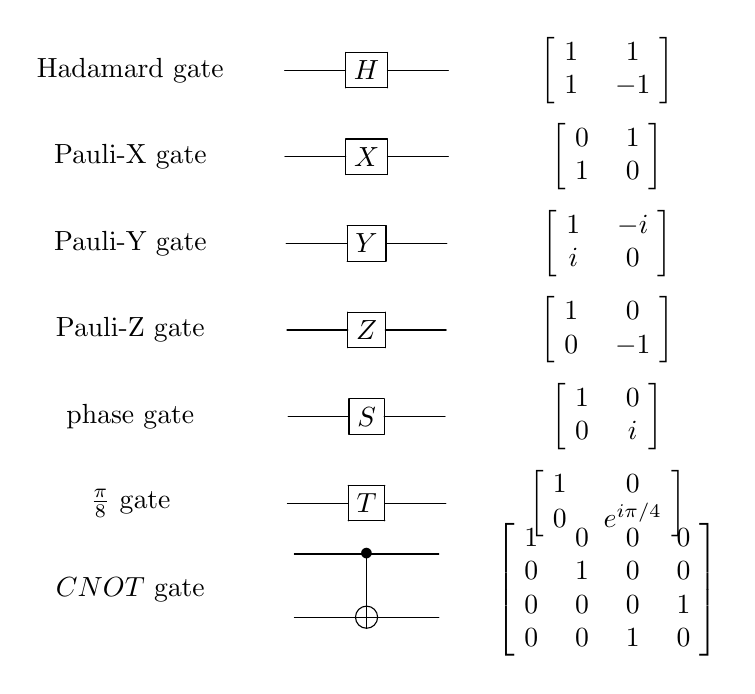
\begin{tikzpicture}
	% $CNOT$
	\node at (7,0){	$CNOT$ gate };
	\node at (10,0){	
		\Qcircuit @C=2.2em @R=1.75em {
		 & \ctrl{1}  & \qw 	 \\
		 &\targ  	 & \qw   \\	    						 
	}};
	\node at (13,0){\vspace{10em}
				$\begin{bmatrix}
					\ 1\ & 0\ & 0\ & 0\ \\
					\ 0\ & 1\ & 0\ & 0\ \\
					\ 0\ & 0\ & 0\ & 1\ \\
					\ 0\ & 0\ & 1\ & 0\ 
				\end{bmatrix}$
	};

		% T
\node at (7,1.1){	$\frac{\pi}{8}$ gate };
\node at (10,1.1){	\Qcircuit @C=2.2em @R=1.75em {
	 & \gate{T}  & \qw 	 \\						 
}};
\node at (13,1.1){\vspace{10em}
			$\begin{bmatrix}
				\ 1\ & 0\  \\
				\ 0\ & e^{i\pi/4}\ \\
			\end{bmatrix}$
};
% phase gate
\node at (7,2.2){	phase gate };
\node at (10,2.2){	
	\Qcircuit @C=2.2em @R=1.75em {
	 & \gate{S}  & \qw 	 \\						 
}};
\node at (13,2.2){\vspace{10em}
			$\begin{bmatrix}
				\ 1\ & 0\  \\
				\ 0\ & i\ \\
			\end{bmatrix}$
};

% Z gate
\node at (7,3.3){	Pauli-Z gate };
\node at (10,3.3){	
	\Qcircuit @C=2.2em @R=1.75em {
	 & \gate{Z}  & \qw 	 \\						 
}};
\node at (13,3.3){\vspace{10em}
			$\begin{bmatrix}
				\ 1\ & 0\  \\
				\ 0\ & -1\ \\
			\end{bmatrix}$
};

% Y gate
\node at (7,4.4){	Pauli-Y gate };
\node at (10,4.4){	
	\Qcircuit @C=2.2em @R=1.75em {
	 & \gate{Y}  & \qw 	 \\						 
}};
\node at (13,4.4){\vspace{10em}
			$\begin{bmatrix}
				\ 1\ & -i\  \\
				\ i\ & 0\ \\
			\end{bmatrix}$
};
% X gate
\node at (7,5.5){	Pauli-X gate };
\node at (10,5.5){	
	\Qcircuit @C=2.2em @R=1.75em {
	 & \gate{X}  & \qw 	 \\						 
}};
\node at (13,5.5){\vspace{10em}
			$\begin{bmatrix}
				\ 0\ & 1\  \\
				\ 1\ & 0\ \\
			\end{bmatrix}$
};
% H
	% IBM Q20
	\node at (7,6.6){	Hadamard gate };
	\node at (10,6.6){	\Qcircuit @C=2.2em @R=1.75em {
		 & \gate{H}  & \qw 	 \\  						 
	}};
	\node at (13,6.6){\vspace{10em}
				$\begin{bmatrix}
					\ 1\ & 1\ \\
					\ 1\ & -1\ 
				\end{bmatrix}$
	};
\end{tikzpicture}
\end{center}

\caption{The symbols of common quantum gates and their matrices }
	\label{common_gates}
\end{figure}	 

}
 \subsubsection{$Quantum \ Circuit$.}
The number of qubits used in quantum circuit is called circuit width $w$. 
The logic dependence graph (see Fig.~\ref{DAG}) of a circuit is obtained by parallelizing 
and layering the circuit by topological sorting. The number of layers that 
can be executed in parallel is called the depth $d$ of the circuit.
As shown in the Fig.~\ref{OriginalCircuit} is a logic circuit ($LC$) generated according to the $openQASM$ program.
Each line represents a qubit, and the gate operation on the line acts on the corresponding qubit.
In this paper, circuits with a depth less than 100 are called small circuits, 
circuits with a depth greater than 1000 are called large circuits, 
and the rest are medium circuits.
The execution order of the circuit is from left to right. 
The depth of the circuit (see Fig.~\ref{OriginalCircuit}) is 6 and the width is 5.
Since the single quantum gate is $local$ \cite{2013Optimization}, 
it is not necessary to consider the single quantum gate in circuit transformation. 
In this paper, the initial mapping is generated by regarding qubit in circuit 
as node and 2-qubits gate as edge. 
The generated logical circuit architecture graph $\mathcal{AG}_{L}=(V_{L},E_{L})$ 
and physical architecture graph $\mathcal{AG}_{P}=(V_{P},E_{P})$ are matched by subgraphs. 
As shown in Fig.~\ref{LAGPAG}(a) is the logical connection graph 
of the original circuit(see Fig.~\ref{OriginalCircuit}),
and Fig.~\ref{LAGPAG}(b) is the partial architecture graph of IBM Q20.
\begin{figure}[h!] 
	\begin{center}
		  {\scalefont{1.0}
	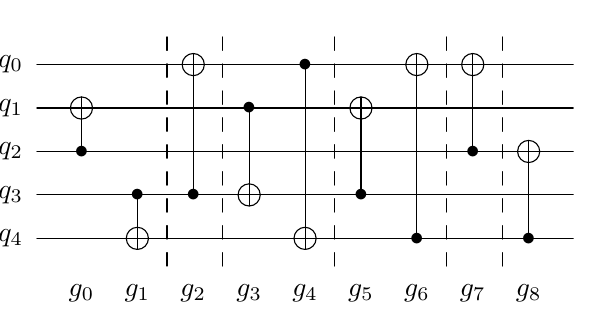
\begin{tikzpicture}
		% \draw[help lines] (0,0) grid (11,7);
		% IBM Q20
		\node at (5.5,5){  \Qcircuit @C=1.2em @R=0.75em {
			\lstick{q_{0}}   &  \qw 				&   \qw  \barrier{4}&\targ 	\barrier{4}	&\qw      		&\ctrl{4}\barrier{4}&   \qw		&\targ\barrier{4} &\targ  \barrier{4}&\qw  &  \qw       \\
			\lstick{q_{1}}   &   \targ      		&   \qw      		&   \qw      		&   \ctrl{2} 	&   \qw      	&   \targ    	&   \qw      	&   \qw       	&   \qw   		&  \qw       \\
			\lstick{q_{2}}   &   \ctrl{-1}  		&   \qw      		&   \qw      		&   \qw      	&   \qw      	&   \qw      	&   \qw     	&   \ctrl{-2} 	&   \targ       &  \qw       \\
			\lstick{q_{3}}   &\qw					&   \ctrl{1}   		&   \ctrl{-3} 		&   \targ    	&   \qw      	&   \ctrl{-2}	&   \qw      	&   \qw       	&   \qw        	&  \qw         \\
			\lstick{q_{4}}   &		\qw				& \targ				& \qw 				&   \qw      	&   \targ    	&   \qw      	&   \ctrl{-4}  	& 	\qw     	&   \ctrl{-2} 	&   \qw			\\
							  &\dstick{g_{0}}		&\dstick{g_{1}}		&\dstick{g_{2}}		&\dstick{g_{3}}	&\dstick{g_{4}} &\dstick{g_{5}} &\dstick{g_{6}} &\dstick{g_{7}} &\dstick{g_{8}}	&   		\\		 
							 &						&					&				&       		& 				& 				& 				&				&   				 
							 }};
	\end{tikzpicture}
	}
	\end{center}					 
	\caption{Original circuit}
	\label{OriginalCircuit}	
	 \end{figure}

	 \begin{figure}[h!] 
		\begin{center}
	{\scalefont{0.5}
		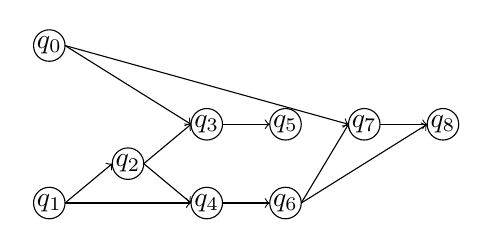
\begin{tikzpicture}							 
	\draw [black,  thin] (3,1) circle [radius=0.2];
	\draw [black,  thin] (3,3) circle [radius=0.2];
	\draw [black,  thin] (4,1.5) circle [radius=0.2];
	\draw [black,  thin] (5,1) circle [radius=0.2];
	\draw [black,  thin] (5,2) circle [radius=0.2];
	\draw [black,  thin] (6,2) circle [radius=0.2];
	\draw [black,  thin] (6,1) circle [radius=0.2];
	\draw [black,  thin] (7,2) circle [radius=0.2];
	\draw [black,  thin] (8,2) circle [radius=0.2];
	% label
	\node at (3,1) {$q_{1}$};
	\node at (3,3) {$q_{0}$};
	\node at (4,1.5) {$q_{2}$};
	\node at (5,1){$q_{4}$};
	\node at (5,2) {$q_{3}$};
	\node at (6,2){$q_{5}$};
	\node at (6,1) {$q_{6}$};
	\node at (7,2) {$q_{7}$};
	\node at (8,2) {$q_{8}$};

	% q1
	\draw [->, thin] (3.2,1) -- (3.8,1.5);
	\draw [->, thin] (3.2,1) -- (4.8,1);
	% q0
	\draw [->, thin] (3.2,3) -- (4.8,2);
	\draw [->, thin] (3.2,3) -- (6.8,2);
	% q2
	\draw [->, thin] (4.2,1.5) -- (4.8,1);
	\draw [->, thin] (4.2,1.5) -- (4.8,2);
	% q3
	\draw [->, thin] (5.2,2) -- (5.8,2);
	% q4
	\draw [->, thin] (5.2,1) -- (5.8,1);
	% q6
	\draw [->, thin] (6.2,1) -- (7.8,2);
	\draw [->, thin] (6.2,1) -- (6.8,2);
	% q7
	\draw [->, thin] (7.2,2) -- (7.8,2);
	\end{tikzpicture}
}
\end{center}
	\caption{The directed acyclic graph(DAG) of original circuit in Fig.~\ref{OriginalCircuit}}
	\label{DAG}
  \end{figure}

\begin{figure}[h!]
	{\scalefont{0.5}
	\begin{center}
	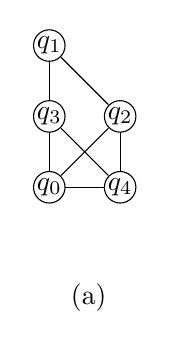
\begin{tikzpicture}
		\node at (0.5,0){(a)};
            % Q20
            \draw [black, thin] (0,1.4) circle [radius=0.2];
            \draw [-,thin] (0.2,1.4) -- (0.7,1.4);
            \draw [black, thin] (0.9,1.4) circle [radius=0.2];
            % label
            \node at (0,1.4) {$q_{0}$};
            \node at (0.9,1.4){$q_{4}$};
            % |
            \draw [-,thin] (0,1.6) -- (0,2.1);
            \draw [-,thin] (0.9,1.6)-- (0.9,2.1);
        
            \draw [black, thin] (0,2.3) circle [radius=0.2];
        
            \draw [black, thin] (0.9,2.3) circle [radius=0.2];
            % label
            \node at (0,2.3) {$q_{3}$};
            \node at (0.9,2.3){$q_{2}$};
            % |
            \draw [-,thin] (0,2.5) -- (0,3.0);
        
            \draw [black, thin] (0,3.2) circle [radius=0.2];
            \draw [-,thin] (0.15,3.05) -- (0.75,2.45);
            % label
            \node at (0,3.2) {$q_{1}$};
        
            %x
        
            \draw [-,thin] (0.15,2.15) -- (0.75,1.55);
			\draw [-,thin] (0.15,1.55) -- (0.75,2.15);
			\label{LLAG}
			\end{tikzpicture}
			\qquad   \qquad
			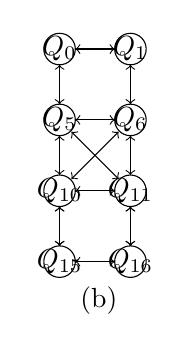
\begin{tikzpicture}
            
                % IBM Q20
            \node at (0.5,0){(b)};
            % Q20
            \draw [black, thin] (0,0.5) circle [radius=0.2];
            \draw [<->,thin] (0.2,0.5) -- (0.7,0.5);
            \draw [black, thin] (0.9,0.5) circle [radius=0.2];
        
            \node at (0,0.5) {$Q_{15}$};
            \node at (0.9,0.5){$Q_{16}$};
            % |
            \draw [<->,thin] (0,0.7) -- (0,1.2);
            \draw [<->,thin] (0.9,0.7) -- (0.9,1.2);
            % |
            \draw [<->,thin] (0,0.7) -- (0,1.2);
            \draw [<->,thin] (0.9,0.7) -- (0.9,1.2);
        
            \draw [black, thin] (0,1.4) circle [radius=0.2];
            \draw [<->,thin] (0.2,1.4) -- (0.7,1.4);
            \draw [black, thin] (0.9,1.4) circle [radius=0.2];
            % label
            \node at (0,1.4) {$Q_{10}$};
            \node at (0.9,1.4){$Q_{11}$};
            % |
            \draw [<->,thin] (0,1.6) -- (0,2.1);
            \draw [<->,thin] (0.9,1.6)-- (0.9,2.1);
        
            \draw [black, thin] (0,2.3) circle [radius=0.2];
            \draw [<->,thin] (0.2,2.3) -- (0.7,2.3);
            \draw [black, thin] (0.9,2.3) circle [radius=0.2];
            % label
            \node at (0,2.3) {$Q_{5}$};
            \node at (0.9,2.3){$Q_{6}$};
            % |
            \draw [<->,thin] (0,2.5) -- (0,3.0);
            \draw [<->,thin] (0.9,2.5)-- (0.9,3.0);
        
            \draw [black, thin] (0,3.2) circle [radius=0.2];
            \draw [<->,thin] (0.2,3.2) -- (0.7,3.2);
            \draw [black, thin] (0.9,3.2) circle [radius=0.2];
            % label
            \node at (0,3.2) {$Q_{0}$};
            \node at (0.9,3.2){$Q_{1}$};
        
            %x
        
            \draw [<->,thin] (0.15,2.15) -- (0.75,1.55);
			\draw [<->,thin] (0.15,1.55) -- (0.75,2.15);
			\label{PPAG}
	\end{tikzpicture}
\end{center}
	}
	\caption{(a)The architecture graph of original circuit in Fig.~\ref{OriginalCircuit}. (b) The partial architecture graph of IBM Q20 }
	\label{LAGPAG}
\end{figure}
	
\begin{figure}[h!] 				
	\centerline{ 
\Qcircuit @C=1.2em @R=1.5em {
							 &  \ctrl{1}  		&     \qw \\
							 &   \targ      		&       \qw   \\	 
							&					&      						 
					}
					  \qquad    \qquad
  \Qcircuit @C=1.2em @R=0.75em {
	 &   \gate{H}  		&\targ 			&\gate{H}     	&    \qw  	 \\
	 &   \gate{H}      	&\ctrl{-1}      &\gate{H} 		&   \qw 	    \\	 
	&					&				& 				&						 
					  }
  }

  \caption{Transformation of gate direction}
  \label{Transformate}
\end{figure}
\begin{figure}[h!] 				
   \centerline{ 
					\Qcircuit @C=1.2em @R=2.05em {
											\lstick{q_{0}} &  \qswap  				&    \rstick{q_{1}} \qw \\
											\lstick{q_{1}} &   \qswap\qwx	   		&     \rstick{q_{0}}  \qw   \\	 
																					&					&      						 
										}
										\qquad    \qquad
\Qcircuit @C=1.2em @R=1.22em {
					   \lstick{q_{0}} 	&  \ctrl{1}  		&  \targ  		&  \ctrl{1}  		&    \rstick{q_{1}} \qw \\
					   \lstick{q_{1}} 	&   \targ      		&  \ctrl{-1}    &   \targ      		&     \rstick{q_{0}}  \qw   \\	 
										&					&				&					&      						 
				   }
					 \qquad    \qquad
 \Qcircuit @C=1.2em @R=0.75em {
	\lstick{q_{0}}  &  \ctrl{1}  		&   \gate{H}  		&\ctrl{1} 			&\gate{H}     	&\ctrl{1}			&    \rstick{q_{1}}\qw  	 \\
	\lstick{q_{1}}  &   \targ      		&   \gate{H}      	&   \targ      		&\gate{H} 		&\targ      		&    \rstick{q_{0}}\qw 	    \\	 
					&					&					&					&       		& 					&						 
					 }
 }

   \caption{Decomposition of a SWAP gate	   }
   \label{Decomposition}
 \end{figure}

\subsection{Hardware Condition}
\subsubsection{Architectures}
This paper mainly discusses the physical circuit of IBM. 
Let $\mathcal{\mathcal{AG}_{P}}=(V_{P},E_{P})$ denote the architecture graph of the physical circuit, 
$V_{P} $ denotes the physical qubit set, 
and $E_{P}$ represents the directed edge that the $CNOT$ gate can execute.
As shown in the Fig.~\ref{IBM}(a) and (b) are the physical architecture graph of the 5-qubits of IBM QX2, 
(c) and (d) are the physical architecture graph of 16-qubits of IBM QX3, 
and (e) are the physical architecture graph of IBM Q20 series. 
The arrow in the figure indicates that the qubit at the beginning of the arrow can control 
the qubit at the end of the arrow, and the 2-qubits gate operation can only be performed between 
qubit with edges connected. 
Since the quantum logic circuit does not consider physical constraints, 
any gate operation can be performed between two non-adjacent logic qubits, 
but IBM physical circuit only supports single quantum gate and $CNOT$ gate between two adjacent qubits. 
Therefore, before the circuit transformation, the circuit is simplified to a circuit with only single 
quantum gate and $CNOT$ gate. This part of the work has been implemented in \cite{2005Mttnen,1995Barenco}. 
\cite{Lloyd1995Almost} is proved that almost all gates of two qubits can be represented by general quantum gates. 
Generally, mapping logic qubit directly to physical qubit can not satisfy the limit of logic circuit, 
and circuit transformation is needed to make quantum gate can be executed on physical devices. 
This process is called circuit transformation in this paper. In this paper, we insert the 
auxiliary gate(SWAP)as shown in the Fig.~\ref{Decomposition},
so that two non-adjacent qubits can be logically swap to adjacent positions, 
or change direction between two adjacent qubits (see Fig.~\ref{Transformate}). 
The introduction of auxiliary gate may lead to errors, 
which may lead to large deviation between the final results and the actual situation. 
The quantum system is easy to interact with the surrounding environment, 
resulting in errors. In the NISQ era, quantum error correction is difficult to achieve. 
Due to the decoherence problem of quantum, the quantum operation needs to be completed in the coherent period, 
and the time of quantum in the coherent state is very short. Therefore, 
it is necessary to improve the parallelism of qubits as much as possible to minimize the depth 
of quantum circuit. This is the focus of this paper. We hope to find a circuit mapping scheme 
with the minimum number of auxiliary gates and the circuit depth in the acceptable time.

\begin{figure}
	{
	\scalefont{0.5}
	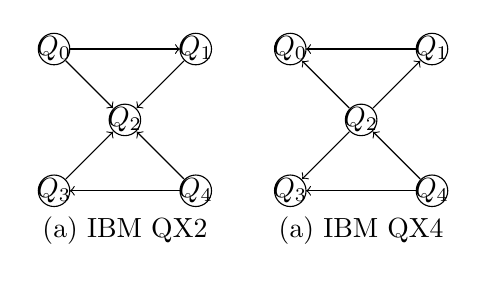
\begin{tikzpicture}
	% \draw[help lines] (0,0) grid (11,3);
		% IBM QX2
	\node at (1.8,0.4){(a) IBM QX2};
	\node at (4.8,0.4){(a) IBM QX4};
	% label
	\node at (0.9,2.7){$Q_{0}$};
	\draw [black, thin] (0.9,2.7) circle [radius=0.2];
	\node at (2.7,2.7){$Q_{1}$};
	\draw [black, thin] (2.7,2.7) circle [radius=0.2];
	\node at (1.8,1.8){$Q_{2}$};
	\draw [black, thin] (1.8,1.8)circle [radius=0.2];
	\node at (0.9,0.9){$Q_{3}$};
	\draw [black, thin] (0.9,0.9) circle [radius=0.2];
	\node at (2.7,0.9){$Q_{4}$};
	\draw [black, thin] (2.7,0.9) circle [radius=0.2];

	
	% -
	\draw [->,thin] (1.1,2.7) -- (2.5,2.7);
	
	\draw [<-,thin] (1.1,0.9) -- (2.5,0.9);

	%x
	\draw [->,thin] (1.05,2.55) -- (1.65,1.95);
	\draw [->,thin] (2.55,2.55) -- (1.95,1.95);
	\draw [->,thin] (1.05,1.05) -- (1.65,1.65);
	\draw [->,thin] (2.55,1.05) -- (1.95,1.65);

		 
		% label
		\node at (3.9,2.7){$Q_{0}$};
		\draw [black, thin] (3.9,2.7) circle [radius=0.2];
		\node at (5.7,2.7){$Q_{1}$};
		\draw [black, thin] (5.7,2.7) circle [radius=0.2];
		\node at (4.8,1.8){$Q_{2}$};
		\draw [black, thin] (4.8,1.8)circle [radius=0.2];
		\node at (3.9,0.9){$Q_{3}$};
		\draw [black, thin] (3.9,0.9) circle [radius=0.2];
		\node at (5.7,0.9){$Q_{4}$};
		\draw [black, thin] (5.7,0.9) circle [radius=0.2];
		
		% -
		\draw [<-,thin] (4.1,2.7) -- (5.5,2.7);
		
		\draw [<-,thin] (4.1,0.9) -- (5.5,0.9);
	
		%x
		\draw [<-,thin] (4.05,2.55) -- (4.65,1.95);
		\draw [<-,thin] (5.55,2.55) -- (4.95,1.95);
		\draw [<-,thin] (4.05,1.05) -- (4.65,1.65);
		\draw [->,thin] (5.55,1.05) -- (4.95,1.65);
	
	\end{tikzpicture}
}
\\
{
	\scalefont{0.5}
		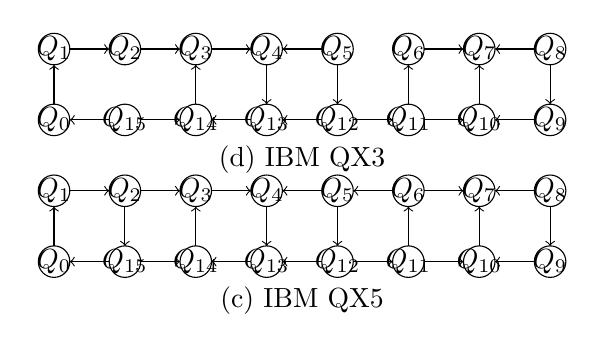
\begin{tikzpicture}
			
	\node at (3.15,0){(c) IBM QX5};
	\node at (3.15,1.8){(d) IBM QX3};
		%QX5
		%-
	\draw [black, thin] (0,2.3) circle [radius=0.2];
	\draw [<-,thin] (0.2,2.3) -- (0.7,2.3);
	\draw [black, thin] (0.9,2.3) circle [radius=0.2];
	\draw [->,thin] (1.1,2.3) -- (1.6,2.3);
	\draw [black, thin] (1.8,2.3) circle [radius=0.2];
	\draw [<-,thin] (2.0,2.3) -- (2.5,2.3);
	\draw [black, thin] (2.7,2.3) circle [radius=0.2];
	\draw [<-,thin] (2.9,2.3) -- (3.4,2.3);
	\draw [black, thin] (3.6,2.3) circle [radius=0.2];
	\draw [->,thin] (3.8,2.3) -- (4.3,2.3);
	\draw [black, thin] (4.5,2.3) circle [radius=0.2];
	\draw [->,thin] (4.7,2.3) -- (5.2,2.3);
	\draw [black, thin] (5.4,2.3) circle [radius=0.2];
	\draw [<-,thin] (5.6,2.3) -- (6.1,2.3);
	\draw [black, thin] (6.3,2.3) circle [radius=0.2];

	% |
	\draw [->,thin] (0,2.5) -- (0,3.0);
	\draw [->,thin] (1.8,2.5) -- (1.8,3.0);
	\draw [<-,thin] (2.7,2.5) -- (2.7,3.0);
	\draw [<-,thin] (3.6,2.5) -- (3.6,3.0);
	\draw [->,thin] (4.5,2.5) -- (4.5,3.0);
	\draw [->,thin] (5.4,2.5) -- (5.4,3.0);
	\draw [<-,thin] (6.3,2.5) -- (6.3,3.0);
	%-
\draw [black, thin] (0,3.2) circle [radius=0.2];
\draw [->,thin] (0.2,3.2) -- (0.7,3.2);
\draw [black, thin] (0.9,3.2) circle [radius=0.2];
\draw [->,thin] (1.1,3.2) -- (1.6,3.2);
\draw [black, thin] (1.8,3.2) circle [radius=0.2];
\draw [->,thin] (2.0,3.2) -- (2.5,3.2);
\draw [black, thin] (2.7,3.2) circle [radius=0.2];
\draw [<-,thin] (2.9,3.2) -- (3.4,3.2);
\draw [black, thin] (3.6,3.2) circle [radius=0.2];

\draw [black, thin] (4.5,3.2) circle [radius=0.2];
\draw [->,thin] (4.7,3.2) -- (5.2,3.2);
\draw [black, thin] (5.4,3.2) circle [radius=0.2];
\draw [<-,thin] (5.6,3.2) -- (6.1,3.2);
\draw [black, thin] (6.3,3.2) circle [radius=0.2];
	
	% label
	\node at (0,0.5){$Q_{0}$};
	\node at (0.9,0.5){$Q_{15}$};
	\node at (1.8,0.5){$Q_{14}$};
	\node at (2.7,0.5){$Q_{13}$};
	\node at (3.6,0.5){$Q_{12}$};
	\node at (4.5,0.5){$Q_{11}$};
	\node at (5.4,0.5){$Q_{10}$};
	\node at (6.3,0.5){$Q_{9}$};

	\node at (0,1.4){$Q_{1}$};
	\node at (0.9,1.4){$Q_{2}$};
	\node at (1.8,1.4){$Q_{3}$};
	\node at (2.7,1.4){$Q_{4}$};
	\node at (3.6,1.4){$Q_{5}$};
	\node at (4.5,1.4){$Q_{6}$};
	\node at (5.4,1.4){$Q_{7}$};
	\node at (6.3,1.4){$Q_{8}$};

		%QX5
		%-
		\draw [black, thin] (0,0.5) circle [radius=0.2];
		\draw [<-,thin] (0.2,0.5) -- (0.7,0.5);
		\draw [black, thin] (0.9,0.5) circle [radius=0.2];
		\draw [->,thin] (1.1,0.5) -- (1.6,0.5);
		\draw [black, thin] (1.8,0.5) circle [radius=0.2];
		\draw [<-,thin] (2.0,0.5) -- (2.5,0.5);
		\draw [black, thin] (2.7,0.5) circle [radius=0.2];
		\draw [<-,thin] (2.9,0.5) -- (3.4,0.5);
		\draw [black, thin] (3.6,0.5) circle [radius=0.2];
		\draw [->,thin] (3.8,0.5) -- (4.3,0.5);
		\draw [black, thin] (4.5,0.5) circle [radius=0.2];
		\draw [->,thin] (4.7,0.5) -- (5.2,0.5);
		\draw [black, thin] (5.4,0.5) circle [radius=0.2];
		\draw [<-,thin] (5.6,0.5) -- (6.1,0.5);
		\draw [black, thin] (6.3,0.5) circle [radius=0.2];
	
		% |
		\draw [->,thin] (0,0.7) -- (0,1.2);
		\draw [<-,thin] (0.9,0.7) -- (0.9,1.2);
		\draw [->,thin] (1.8,0.7) -- (1.8,1.2);
		\draw [<-,thin] (2.7,0.7) -- (2.7,1.2);
		\draw [<-,thin] (3.6,0.7) -- (3.6,1.2);
		\draw [->,thin] (4.5,0.7) -- (4.5,1.2);
		\draw [->,thin] (5.4,0.7) -- (5.4,1.2);
		\draw [<-,thin] (6.3,0.7) -- (6.3,1.2);
		%-
	\draw [black, thin] (0,1.4) circle [radius=0.2];
	\draw [->,thin] (0.2,1.4) -- (0.7,1.4);
	\draw [black, thin] (0.9,1.4) circle [radius=0.2];
	\draw [->,thin] (1.1,1.4) -- (1.6,1.4);
	\draw [black, thin] (1.8,1.4) circle [radius=0.2];
	\draw [->,thin] (2.0,1.4) -- (2.5,1.4);
	\draw [black, thin] (2.7,1.4) circle [radius=0.2];
	\draw [<-,thin] (2.9,1.4) -- (3.4,1.4);
	\draw [black, thin] (3.6,1.4) circle [radius=0.2];
	\draw [<-,thin] (3.8,1.4) -- (4.3,1.4);
	\draw [black, thin] (4.5,1.4) circle [radius=0.2];
	\draw [->,thin] (4.7,1.4) -- (5.2,1.4);
	\draw [black, thin] (5.4,1.4) circle [radius=0.2];
	\draw [<-,thin] (5.6,1.4) -- (6.1,1.4);
	\draw [black, thin] (6.3,1.4) circle [radius=0.2];
		
		% label
		\node at (0,2.3){$Q_{0}$};
		\node at (0.9,2.3){$Q_{15}$};
		\node at (1.8,2.3){$Q_{14}$};
		\node at (2.7,2.3){$Q_{13}$};
		\node at (3.6,2.3){$Q_{12}$};
		\node at (4.5,2.3){$Q_{11}$};
		\node at (5.4,2.3){$Q_{10}$};
		\node at (6.3,2.3){$Q_{9}$};
	
		\node at (0,3.2){$Q_{1}$};
		\node at (0.9,3.2){$Q_{2}$};
		\node at (1.8,3.2){$Q_{3}$};
		\node at (2.7,3.2){$Q_{4}$};
		\node at (3.6,3.2){$Q_{5}$};
		\node at (4.5,3.2){$Q_{6}$};
		\node at (5.4,3.2){$Q_{7}$};
		\node at (6.3,3.2){$Q_{8}$};
	\end{tikzpicture}
}
{\scalefont{0.5}
	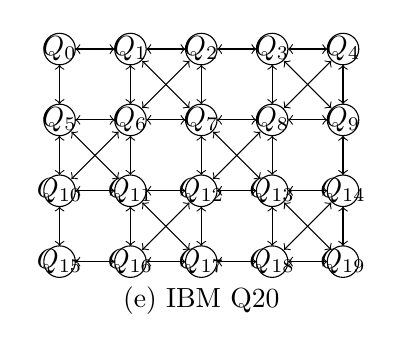
\begin{tikzpicture}
	
		% IBM Q20
		\node at (1.8,0){(e) IBM Q20};
	% Q20
	\draw [black, thin] (0,0.5) circle [radius=0.2];
	\draw [<->,thin] (0.2,0.5) -- (0.7,0.5);
	\draw [black, thin] (0.9,0.5) circle [radius=0.2];
	\draw [<->,thin] (1.1,0.5) -- (1.6,0.5);
	\draw [black, thin] (1.8,0.5) circle [radius=0.2];
	\draw [<->,thin] (2.0,0.5) -- (2.5,0.5);
	\draw [black, thin] (2.7,0.5) circle [radius=0.2];
	\draw [<->,thin] (2.9,0.5) -- (3.4,0.5);
	\draw [black, thin] (3.6,0.5) circle [radius=0.2];

	\node at (0,0.5) {$Q_{15}$};
	\node at (0.9,0.5){$Q_{16}$};
	\node at (1.8,0.5){$Q_{17}$};
	\node at (2.7,0.5){$Q_{18}$};
	\node at (3.6,0.5){$Q_{19}$};
	% |
	\draw [<->,thin] (0,0.7) -- (0,1.2);
	\draw [<->,thin] (0.9,0.7) -- (0.9,1.2);
	\draw [<->,thin] (1.8,0.7) -- (1.8,1.2);
	\draw [<->,thin] (2.7,0.7) -- (2.7,1.2);
	\draw [<->,thin] (3.6,0.7) -- (3.6,1.2);

	\draw [black, thin] (0,1.4) circle [radius=0.2];
	\draw [<->,thin] (0.2,1.4) -- (0.7,1.4);
	\draw [black, thin] (0.9,1.4) circle [radius=0.2];
	\draw [<->,thin] (1.1,1.4) -- (1.6,1.4);
	\draw [black, thin] (1.8,1.4)circle [radius=0.2];
	\draw [<->,thin] (2.0,1.4) -- (2.5,1.4);
	\draw [black, thin] (2.7,1.4) circle [radius=0.2];
	\draw [<->,thin] (2.9,1.4) -- (3.4,1.4);
	\draw [black, thin] (3.6,1.4) circle [radius=0.2];
	% label
	\node at (0,1.4) {$Q_{10}$};
	\node at (0.9,1.4){$Q_{11}$};
	\node at (1.8,1.4){$Q_{12}$};
	\node at (2.7,1.4){$Q_{13}$};
	\node at (3.6,1.4){$Q_{14}$};
	% |
	\draw [<->,thin] (0,1.6) -- (0,2.1);
	\draw [<->,thin] (0.9,1.6)-- (0.9,2.1);
	\draw [<->,thin] (1.8,1.6) -- (1.8,2.1);
	\draw [<->,thin] (2.7,1.6) -- (2.7,2.1);
	\draw [<->,thin] (3.6,1.6) -- (3.6,2.1);

	\draw [black, thin] (0,2.3) circle [radius=0.2];
	\draw [<->,thin] (0.2,2.3) -- (0.7,2.3);
	\draw [black, thin] (0.9,2.3) circle [radius=0.2];
	\draw [<->,thin] (1.1,2.3) -- (1.6,2.3);
	\draw [black, thin] (1.8,2.3)circle [radius=0.2];
	\draw [<->,thin] (2.0,2.3) -- (2.5,2.3);
	\draw [black, thin] (2.7,2.3) circle [radius=0.2];
	\draw [<->,thin] (2.9,2.3) -- (3.4,2.3);
	\draw [black, thin] (3.6,2.3) circle [radius=0.2];
	% label
	\node at (0,2.3) {$Q_{5}$};
	\node at (0.9,2.3){$Q_{6}$};
	\node at (1.8,2.3){$Q_{7}$};
	\node at (2.7,2.3){$Q_{8}$};
	\node at (3.6,2.3){$Q_{9}$};
	% |
	\draw [<->,thin] (0,2.5) -- (0,3.0);
	\draw [<->,thin] (0.9,2.5)-- (0.9,3.0);
	\draw [<->,thin] (1.8,2.5) -- (1.8,3.0);
	\draw [<->,thin] (2.7,2.5) -- (2.7,3.0);
	\draw [<->,thin] (3.6,2.5) -- (3.6,3.0);

	\draw [black, thin] (0,3.2) circle [radius=0.2];
	\draw [<->,thin] (0.2,3.2) -- (0.7,3.2);
	\draw [black, thin] (0.9,3.2) circle [radius=0.2];
	\draw [<->,thin] (1.1,3.2) -- (1.6,3.2);
	\draw [black, thin] (1.8,3.2)circle [radius=0.2];
	\draw [<->,thin] (2.0,3.2) -- (2.5,3.2);
	\draw [black, thin] (2.7,3.2) circle [radius=0.2];
	\draw [<->,thin] (2.9,3.2) -- (3.4,3.2);
	\draw [black, thin] (3.6,3.2) circle [radius=0.2];
	% label
	\node at (0,3.2) {$Q_{0}$};
	\node at (0.9,3.2){$Q_{1}$};
	\node at (1.8,3.2){$Q_{2}$};
	\node at (2.7,3.2){$Q_{3}$};
	\node at (3.6,3.2){$Q_{4}$};

	%x
	\draw [<->,thin] (1.05,0.65) -- (1.65,1.25);
	\draw [<->,thin] (1.05,1.25) -- (1.65,0.65);
	\draw [<->,thin] (2.85,0.65) -- (3.45,1.25);
	\draw [<->,thin] (2.85,1.25) -- (3.45,0.65);

	\draw [<->,thin] (1.05,2.45) -- (1.65,3.05);
	\draw [<->,thin] (1.05,3.05) -- (1.65,2.45);
	\draw [<->,thin] (2.85,2.45) -- (3.45,3.05);
	\draw [<->,thin] (2.85,3.05) -- (3.45,2.45);

	\draw [<->,thin] (0.15,2.15) -- (0.75,1.55);
	\draw [<->,thin] (0.15,1.55) -- (0.75,2.15);
	\draw [<->,thin] (1.95,2.15) -- (2.55,1.55);
	\draw [<->,thin] (1.95,1.55) -- (2.55,2.15);
	\end{tikzpicture}
}
\caption{IBM QX architectures}
\label{IBM}
\end{figure}

\section{Problem Analysis}
\label{Problem Analysis}
The goal of this paper is to find a circuit mapping scheme with the minimum number of auxiliary gates 
and the minimum circuit depth in the acceptable time, 
so that the input circuit can satisfy the physical circuit constraints.
\subsubsection{Problem in qubit Mapping}
A quantum circuit transformation problem mainly includes the following four steps, 
among which the third step of $qubits$ $assignment$ and the fourth step of qubit routing 
problem are both NP-comple\cite{2018QubitSiraichi}
\begin{enumerate}
	\item Convert programming language into logical quantum circuit.
	\item Decomposes the circuit into basic gates. 
	Single qubit gates and $CNOT$ gates are used as basic gates, 
	because they are commonly used to implement any quantum circuit 
	and are supported by the IBM QX architecture.
	\item The initial mapping $\tau$ has an important impact on the subsequent 
	addition of auxiliary gates. In this paper, we use the subgraph isomorphism 
	algorithm to get a logical architecture graph that satisfies 
	the quantum physical circuit as much as possible. Since most quantum 
	logic architecture graph can not find a perfect mapping on the physical architecture graph, 
	we try to satisfy as many nodes as possible.

	It will change the mapping relations $\tau$ that the original mapping inserts SWAP gates. 
	Mapping is a injective function
	$\tau:q \rightarrow \ Q $.
	If two mappings are equal $\tau(q_{i})=\tau(q_{j})$, if and only if $i=j$.
	\item The task of modifying the circuit to match the memory layout of 
	a particular quantum computer is called the qubit routing problem~\cite{Cowtan2019}. 
	Since quantum algorithms are usually designed without referring to 
	the connectivity constraints of any specific hardware, routing problems 
	need to be solved before the implementation of quantum circuits. 
	Therefore, qubit routing forms a necessary stage of any compiler 
	for quantum software.

	Given the logic circuit $LC$, physical structure $\mathcal{AG}_{P}$, 
	and an initial mapping $\tau$, $CNOT$ gate $g=\left \langle q_{i},q_{j}\right \rangle $, 
	if gate $G$ is executable, then $\left \langle\tau(q_{i}),\tau(q_{j})\right \rangle $ 
	is a directed edge on $\mathcal{AG}_{P}$.
\begin{example}
	Fig.~\ref{LAGPAG}(a) is the logical structure of Fig.~\ref{OriginalCircuit}, 
	Fig.~\ref{LAGPAG}(b) is the partial architecture graph of IBM Q20, and initial mapping is 
	$\tau=\{q_{0}\rightarrow \ Q_{10},q_{1}\rightarrow \ Q_{0},
			q_{2}\rightarrow \ Q_{6},q_{3}\rightarrow \ Q_{5},q_{4}\rightarrow \ Q_{11}\}$.
			$g_{0}=\left \langle q_{2},q_{1}\right \rangle $ is executable, since 
			$\left \langle \tau(q_{2}),\tau(q_{2})\right \rangle =\left \langle Q_{5},Q_{0}\right \rangle $ exists in $\mathcal{AG}_{P}$.
	But $g_{3}=\left \langle q_{1},q_{3}\right \rangle $ is not executable, since 
	$\left \langle \tau(q_{1}),\tau(q_{3})\right \rangle =\left \langle Q_{0},Q_{6}\right \rangle $  does not exist in $\mathcal{AG}_{P}$.
\end{example}

\end{enumerate}

\section{Solution}
\label{Solution}
The program proposed in this paper mainly includes preprocessing, 
initial mapping, 
and minimum SWAP algorithm based on Tabu Search and  $A^{*}$ algorithm.
\subsection{Preprocessing}
Before the transformation of the SWAP circuit based on Tabu Search, 
we need to preprocess it to get more convenient data to shorten our search time and space.
In the preprocessing stage, we first adjust the circuit of the input openQASM 
program to shorten the life cycle of qubits, then convert the openQASM code 
into a layered form, and generate a logical dependency graph($DAG$) and logical architecture graph($LCG$),
 and then read 
the physical architecture graph into the memory in the specified format, then use BFS to calculate 
the shortest distance between each node on the architecture graph.
\subsubsection{Circuit Adjustment}
In order to shorten the life cycle of qubits and improve the parallelism of qubits, 
we use a layered method \cite{2019Zhang} to analyze the life cycle of qubits, 
and pack the operations that can be executed in parallel into a $bundle$, forming a layered bundle format.
A conversion method is designed to use the layered bundle format to determine 
which operations can be moved, which reduces the life cycle of these qubits.
The algorithm reduces the error rate of quantum programs by 11\%. 
On most quantum workloads, the longest qubit lifetime and the average qubit lifetime 
can be reduced by more than 20\%, and the execution time of some quantum programs can also be reduced.
\subsubsection{Shortest Distance}
As long as the physical architecture graph is determined, 
the shortest distance between two qubits can be calculated. 
In this paper, the shortest distance matrix $dist[i][j]$ is calculated by $Floyd-Warshall$ algorithm, 
which represents the shortest distance from $Q_{i}$ to $Q_{j}$, 
and the distance of each edge is 1. 
For IBM QX2, QX3, QX4, QX5, the SWAP operation needs 7 gates 
(3 $CNOT$ gates and 4 $H$ gates). 
Only 4 $H$ gates are needed to change direction between two adjacent qubits. 
For a $CNOT$ gate $\left \langle  q_{i},q_{j} \right \rangle $,
and two qubits are mapped to $Q_{i}$ and $Q_{j}$ respectively, $\ \tau(q_{i})=Q_{i},\ \tau(q_{j})=Q_{j}$, 
then the cost of executing $g$ under the shortest distance path is $cost_{cnot}(q_{i},q_{j})=7 \times( dist[i][j]-1)$.
If they move to adjacent positions, but there is no edge from $Q_{i}$ to $Q_{j}$,
they need to add 4 $H$ gates to adjust their directions.
 Then the cost between them is $cost_{cnot}(q_{i},q_{j})=3 \times( dist[i][j]-1)$.
In IBM Q20 structure, all the edges are bidirectional. 
The SWAP operation requires 3 gates (3 $CNOT$ gates), 
and there is no need to change the direction. 
Then the calculation formula for IBM Q20 structure is $cost_{cnot}(q_{i},q_{j})=3 \times( dist[i][j]-1)$
The time complexity of this step is $O (N^{3})$.
\begin{example}
	Taking the QX5 structure as an example, 
suppose there is a $CNOT$ gate $g=\left \langle  q_{i}, q_{j} \right \rangle $, \ $q_{i}$ is mapped to $Q_{1}$, 
 $q_{j}$ is mapped to $Q_{14}$, 
and the shortest distance between them  is $dist[1][14]=3$.
There are three shortest paths to move $Q_{1}$ to the adjacent position of $Q_{14}$:
$\Pi=\{\pi_{0},\pi_{1},\pi_{2}\}$
$\pi_{0}={Q_{1}\rightarrow Q_{2} \rightarrow Q_{3} \leftarrow Q_{14}}$,
$\pi_{1}={Q_{1}\rightarrow Q_{2} \rightarrow Q_{15} \rightarrow Q_{14}}$,
$\pi_{2}={Q_{1}\rightarrow Q_{0} \rightarrow Q_{15} \rightarrow Q_{14}}$.
Their costs are 
$cost_{\pi_{0}}=18,\ cost_{\pi_{1}}=14,\ cost_{\pi_{2}}=14$, respectively.
\end{example}

\subsubsection{Circuit Layering}
The SWAP minimization algorithm based on Tabu Search or the $A^{*}$ algorithm 
traverses each level of quantum gate search that can be executed in parallel.
Thus, we layer the adjusted circuit, 
traverse the entire program sequentially, 
and add gates that can be executed in parallel to one layer, 
otherwise a new layer is added. 
The $CNOT$ gate is represented by $\left \langle q,q^{'}\right \rangle $, $q$ is the control qubit, and $q^{'}$ is the target qubit.
$L(LC)=\{\mathcal{L}_{0},\mathcal{L}_{1},...,\mathcal{L}_{n}\}$ represents the layered circuit, 
$\mathcal{L}_{i}, \ (0 \le i \le n) $ represents a quantum gates set that can be executed in parallel.
The quantum gates set separated by the dotted line in the Fig.~\ref{OriginalCircuit}.
 $\mathcal{L}_{0}={g_{0},g_{1}},\mathcal{L}_{1}={g_{2}},
 \mathcal{L}_{2}={g_{3},g_{4}},\mathcal{L}_{3}={g_{5},g_{6}},\mathcal{L}_{4}={g_{7}},\mathcal{L}_{5}={g_{8}}$.

At the same time, we generate circuit architecture graph $\mathcal{AG_{L}}=(V_{L},E_{L})$,
 which is an undirected graph, $V_{L}$ contains the vertex and the degree of the vertex, 
and $E_{L}$ represents the undirected edge that the $CNOT$ gate can execute.
\subsection{Initial Mapping}
It has been proved that the initial mapping has an important influence on $qubits $  
$ assignment$, 
and the subgraph isomorphism can be reduced to $qubits$ $ assignment$, so we want to use the subgraph 
isomorphism algorithm to find an initial mapping which is closer to the optimal.
In the physical architecture graph, it is almost impossible to find a subgraph that exactly 
matches the logical architecture graph, so we hope to find a partial mapping that can maximize the match. 
$SubgraphCompare$\cite{Sun2020} compares several current better subgraph isomorphism algorithm combinations, 
it shows that using the filtering and sorting ideas of GraphQL algorithm to process 
candidate nodes, the local candidate calculation method based on 
set intersection to enumerate the results is the best.
Since $SubgraphCompare$ used in this paper is only suitable for 
fully connected subgraph isomorphism, 
there may be no 2-qubit gate operation between one qubit and other qubits in our circuit.
 The architecture graph formed in this way cannot use $SubgraphCompare$ 
 of this paper to generate part of the initial mapping, 
 because the subgraph matching will first match the node with the largest degree, 
 and we hope to minimize the impact on the logical dependency graph. 
 Therefore, we artificially connect the qubit with a degree of 0 in the logic architecture graph
to the qubit with the largest degree.

We use the algorithm (GraphQL) recommended in \cite{Sun2020} for partial subgraph isomorphism.
The logical architecture graph $\mathcal{AG_{L}}$ 
and the physical architecture graph $\mathcal{AG_{P}}$ generated by the preprocessing process 
are regarded as an undirected graph as input, and then the combined subgraph isomorphism algorithm $SubgraphCompare$ is executed. 
The output of the improved combined subgraph isomorphism algorithm is a file containing all the isomorphism processes.
Since only a small number of nodes may be matched during the isomorphism process, we finally select only the case 
with the most isomorphism nodes as the result of the combined subgraph isomorphism.
Then we complete the unmapped nodes in the partial mapping based on the connectivity of 
the nodes or the degree of the nodes. 
The mapping completion algorithm based on node connectivity is shown in Algorithm \ref{algorithm_initial}.

The input of Algorithm \ref{algorithm_initial} is a target graph ($\mathcal{AG}_{P}$), 
query graph ($\mathcal{AG}_{L}$), and the current mapping relations $T$.
First initialize an empty queue $Q$, which stores unmatched nodes in the map $\tau \in T$ .
Then it traverses $\tau$ and adds the unmatched nodes to the queue. 
The remaining unmatched points we want to try to map them with the nodes that are not 
matched in the more concentrated area of $\mathcal{AG}_{P}$.
That is, 
the final mapping relations can be a dense in the target graph, 
which can reduce subsequent SWAP operations. 
At the beginning, we also tried to randomly match the remaining unmatched nodes, 
but this may lead to isomorphism to a position far away from other nodes, 
adding subsequent auxiliary gate operations.
In the query graph, if the unmatched point has an edge adjacent to the matched point, 
it will be matched to its adjacent position first, 
and if the adjacent position has been matched, 
it will be matched to the adjacent unmatched node.
Finally it gets all the processed candidate initial mappings and outputs them to a file.


Lines 2-7 are to calculate the maximum number of qubits $ml$ that can be matched in the mapping relations 
between logical qubits and physical Qubits obtained by the $SubgraphCompare$ algorithm.
Lines 8-49 are to complete the logical qubit unmapped nodes in the mapping scheme with the number 
of matches equal to $ml$ in the mapping relations, and we use the greedy strategy to allocate.
Line 11, we initialized an empty queue $Q$, which stores unmapped logical qubits.
Lines 12-18, we will traverse the map and add the unmapped qubit to $Q$.
Line 20, loop until $Q$ becomes empty, and all logical qubits are mapped to physical Qubits.
We take out the first element in $Q$. 
Line 21 and 22 are respectively to get the adjacency matrix of $\mathcal{AG}_{P}$ and $\mathcal{AG}_{L}$. 
Line23 is to initializes an empty map $tm$, and the keys are sorted in descending order. 
The key consists of the number of nodes that are connected to $qId$ in the adjacency 
matrix and have been mapped in the current mapping scheme and the nodes constitute a unique key.
Lines 25-31 are to traverse the point $m$ connected to $qId$ in the adjacency matrix. 
If the node $m$ has not been mapped in the map mapping, the node is stored in the $tm$.
Line 32-47 is to traverse the $tm$, select the node with the largest number of 
connections to $qId$ in the $tm$, and it has been mapped to the node ($tm.firstValue$) 
on the physical architecture graph.
The $tId$ in line 33 is the node with the largest number of $qId$ connections 
corresponding to the node on the physical architecture graph.
Line 35 is to remove the object to be matched in the $tm$ from the $tm$.
Lines 36-43 are to select the node adjacent to the $tId$ in the adjacency matrix of the $tId$, 
and map the $qId$ to the node.
\begin{algorithm}  
	\label{algorithm_initial}
	\caption{initial mapping algorithm based on GraphQL}  
	\LinesNumbered  
	\KwIn{$\mathcal{AG_{L}}$: The architecture of logical circuit \\ 
	$\mathcal{AG_{P}}$: The architecture of physical circuit\\
	$T$: A partial mapping set obtained by $SubgraphCompare$  \\
	}
	\KwOut{result: A collection of mapping relations between $\mathcal{AG_{L}}$ and $\mathcal{AG_{P}}$}  
	\textbf{Initialize} result$=\emptyset$ ;\\
		$ml  \leftarrow 0$; The most mapped length in mappings		\\
		\For{$\tau \in T$}{
			\If{ml $\textless $ $\tau$.length}{
				$ml \leftarrow$ $\tau$.length;
			}
		}		
	\For{$\tau$ $\in$ $T$}{
		\If{ml=$\tau$.length}{
			result.add($\tau$);\\
			$Q \leftarrow $ initial an empty unmapped node Queue \\
			$i \leftarrow  1$; \\ 
			\While{i$\leq$$\tau$.length}{
				\If{$\tau$[i]=-1}{
					$Q \leftarrow {i}$;
				}
				$i \leftarrow i+1$;
			}
			\While{Q is not empty}{
				int  $qId \leftarrow$ Q.poll();\\
				$targetAdj \leftarrow$ $\mathcal{AG_{P}}$.adjacencyMatrix(); 	\\
				$queryAdj \leftarrow$ $\mathcal{AG_{L}}$.adjacencyMatrix();	\\
				$tm \leftarrow$ initial an empty  map \\
				$m \leftarrow 1$; \\
				\While{m $\leq$ queryAdj[qId].length}{
					\If{$\tau$[m]$\neq$-1}{
						$tm \leftarrow tm \cup$ \\ $\{queryAdj[qId][m] + "-" + \tau[m], m\}$;	
					}
					$m \leftarrow m+1$;
				}
				\While{tm is not empty}{
					$tId \leftarrow$ $\tau$[tm.firstValue]; \\
					$k \leftarrow 0$; \\
					$tm \leftarrow tm\backslash tm.first()$; \\
					\While{ k $\textless$ targetAdj[tId].length}{
						\If{(targetAdj[tId][k]  $\neq$-1 or targetAdj[k][tId]  $\neq$ -1)\\
						 and not $\tau$.contains(k)}{
							 $\tau[qId] \leftarrow k$; \\
							 break;
						 }
						  $k \leftarrow k+1$;
					}
					\If{k $\neq$ targetAdj[tId].length}{
						break;
					}
				}
			}
		}
	}
	\end{algorithm}
	\begin{example}
		Following the previous example, 
we first use the combined subgraph isomorphism algorithm for the logical architecture graph
(see Fig.~\ref{LAGPAG}(a)) and physical architecture graph (see Fig.~\ref{IBM}(e)) 
to obtain the partial mapping result set $T=\{\tau_{0},\tau_{1},...,\tau_{n}\}$ , 
and then we use one of the partial mapping as an example
$\tau_{i}=\{q_{0}\rightarrow Q_{10},q_{1}\rightarrow -1,
	q_{2}\rightarrow Q_{6},q_{3}\rightarrow Q_{5},q_{4}\rightarrow Q_{11}\}, \ 0 \le i \textless n$. 
	$q_{1}\rightarrow -1$ means that $q_{1}$ is not mapped to the physical structure in the subgraph isomorphism stage,
	so we need to perform mapping completion. 
	The algorithm \ref{algorithm_initial} completion strategy is to find the part of the mapping with
	the maximum mapped nodes in $T$ and perform the mapping completion as the initial mapping.
	In this example, the maximum number of mapped nodes is four. 
	Next, we demonstrate that $\tau_{i}$ is mapped and completed, 
	and the unmapped nodes in $\tau_{i}$ are added to the queue $Q, \ Q=\{q_{1}\}$, 
	and the loop ends until $Q$ is empty. 
	We Take the first element of $Q$ and put it in $qId$, 
	then get the adjacency matrix of the query graph and the target graph, 
	traverse the node $q_{m}$ connected to $qId$ in the adjacency matrix, 
	if the node $q_{m}$ is matched, then we put $q_{m}$ into the map, 
	The key of the map is the number of connections between $q_{m}$ and $qId$ + "-" + $\tau_{i}(q_{m})$,
	 the value is $q_{m}$, and the keys are sorted in descending order. 
	 Then we get $tm=[\{'0-5',q_{3}\},\{'-1-6',q_{2}\},\{'-1-11',q_{4}\},\{'-1-10',q_{0}\}]$, 
	 Then traverse the $tm$ and take out the $value=q_{3}$ of the elements in the $tm$, 
	 calculate the value $tId=Q_{5}$ of $q_{m}$ in the current mapping $\tau_{i}(q_{3})$, 
	 and map $qId$ to the node connected to $tId$ and not yet mapped. 
	 If the nodes connected to $tId$ have been mapped, 
	 the loop continues. In this example, it can be directly mapped to $Q_{0}$. In the end, we get 
	 $ \tau_{i}=\{q_{0}\rightarrow \ Q_{10},q_{1}\rightarrow \ 0,
	q_{2}\rightarrow \ Q_{6},q_{3}\rightarrow \ Q_{5},q_{4}\rightarrow \ Q_{11}\}$.
	\end{example}
\subsection{Swap Minimization}
\subsubsection{Tabu Search}
Tabu Search algorithm is a type of heuristic algorithm. 
The disadvantage of heuristic algorithm is that it thinks that the local optimal is the global optimal. 
There is a Tabu table in the Tabu Search to avoid falling into the local optimal.
The circuit transformation operation in this paper mainly relies on 
the idea of tabu search algorithm, 
aiming to solve the large-scale circuit that the current algorithm is difficult to handle, 
and hope to get a result closer to the optimal solution in a short time.
There are mainly the following objects in Tabu Search: neighborhood fields, neighborhood action, 
Tabu table, candidate set sum, Tabu object, evaluation function, and amnesty rules.
All the edges that can be swapped in the current map are the neighborhood fields in Tabu thinking.
The recently reached state is added to the Tabu table, 
and objects in the Tabu table will not be searched as much as possible. 
The Tabu table in this paper is just in line with our parallel thinking. 
In order to increase the parallelism of quantum circuits, we will give priority to inserting auxiliary operations 
that can be executed in parallel. We try not to use the recently operated qubits as much as possible, 
which are added to the Tabu table, in the same time.
The candidate set is to select several neighborhood objects with the best target value or evaluation value from the neighborhood fields
to join the candidate set. It can be obtained by observation that many SWAP operations are meaningless, 
so in order to save search space, we should perform pruning.
Only the swap of edges adjacent to the gate node with at least one edge is meaningful, 
so our neighborhood fields is the shortest path on the physical architecture graph of the gates. 
Their qubits are not adjacent to the current 
layer, and the edges on these shortest paths are all part of the neighborhood fields.
The Tabu object is the object in the Tabu table.
The evaluation function is to select an SWAP evaluation formula from the candidate set, 
generally taking the objective function as the evaluation function.
The evaluation function is to satisfy some gate mapping operations, 
and the number of SWAP gates added should be small, and the depth of the entire circuit should be small.
The amnesty rule is that when all objects in the candidate set are Tabu, 
or after one object is Tabu, the target value will be greatly reduced. 
In order to achieve the global optimal, the Tabu object can be added to the candidate set. 
As shown in Algorithm \ref{algorithm_Tabu}.

The calculation of the neighborhood fields is shown in Algorithm \ref{algorithm_neighborhood}. 
The input are the current circuit mapping parent $\tau_{p}$, physical Qubits to logical qubits mapping $qubits$, 
logical qubits to physical Qubits mapping $locations$, the current layer list of all gates currentLayers $cl$, 
all the gates nextLayer of the next layer $nl$, and the output is a candidate set of the current mapping, 
The mapping generated by a transformation, where the physical mapping and the logical mapping 
are changed synchronously. $E_{w}$ is the edge of all the shortest paths in the physical architecture 
graph of all gates in the current layer. The weight of the edge is the number of times each edge appears 
in the path. If there are multiple edges reachable in the same shortest distance, 
we will choose the path with the largest total weight in all the shortest paths, 
in the lines 8-18.
Lines 22-37 is to swap all the edges of this path and add them to the candidate set, 
and calculate the cost of each candidate.

\begin{example}
	Under the mapping $\tau_{i}=\{q_{0}\rightarrow \ Q_{10},q_{1}\rightarrow \ 0,
q_{2}\rightarrow \ Q_{6},q_{3}\rightarrow \ Q_{5},q_{4}\rightarrow \ Q_{11}\}$, 
for $L_{0}=\{g_{0},g_{1}\}$, $dist_{cnot}(g_{0})=7,\ dist_{cnot}(g_{1})=7$. 
Gate $g_{1}$ can be executed directly under the $\tau_{i}$ mapping, so it is directly deleted from $L_{0}$.
But $g_{0}$ cannot be executed under the mapping $\tau_{i}$, 
so circuit transformation is required. 
First, we need to calculate the field, 
and add the edge of the shortest path of the gate that cannot be executed in 
$L_{0}$ to the number of occurrences of the same edge of $E_{w}$ as the weight of the edge.
Now the gate that cannot be executed in $L_{0}$ is $g_{0}$. 
Its shortest path is $T=\{\{Q_{6}\rightarrow Q_{1} \rightarrow Q_{0} \},\{Q_{6}\rightarrow Q_{5} \rightarrow Q_{0} \}\}$
$E_{w}=\{\left \langle Q_{6},Q_{1}\right \rangle,\ \left \langle Q_{1},Q_{0}\right \rangle,\ 
\left \langle Q_{6},Q_{5}\right \rangle,\ \left \langle Q_{5},Q_{0}\right \rangle,\ 
\}$, and then traverse the shortest path to calculate the path with the highest weight, 
$w_{\pi_{0}}=2, \ w_{\pi_{0}}=2$. The two weights are equal to take the former.
Then the edges on the swap path are added to the candidate set, 
so the current candidate set is $\{SWAP(Q_{6},Q_{1}),\ SWAP(Q_{1},Q_{0}) \}$.
\end{example}
\begin{algorithm}  
	\label{algorithm_neighborhood}
	\caption{Calculate the neighborhood fields }  
	\LinesNumbered  
	\KwIn{$p$: The current circuit's solution\\ 
	$dist$: The shortest paths of physical architecture\\
	$qubits$: The mapping from physical Qubits to logic qubits \\
	$locations$: The mapping from logic qubits to physical Qubits \\
	$cl$: Gates included in the current layer of circuits \\
	$nl$: Gates included in the next layer of circuits \\
	}
	\KwOut{$results$: The set of candidate solution }  
	\textbf{Initialize}  $results \leftarrow$ $\emptyset$;\\
					$E_{w} \leftarrow$ Calculate the weight of each edge\\
					\For{l $\in $ cl}{
						$l_{1} \leftarrow locations[l.control]$;\\
						$l_{2} \leftarrow locations[l.target]$;\\
						$distance  \leftarrow  dist[l_{1}][l_{2}]$;\\
						$ml$ $\leftarrow 0 $;$sum \leftarrow 0$ ;$path\_index \leftarrow -1$;\\
						\For{path $\in$ distance.paths}{
							\For{edge $\in$ path}{
								\If{$E_{w}$.contains(edge)}{
									$e  \leftarrow$ $E_{w}.findEqualWithEdge(edge)$;\\
									$sum \leftarrow sum + e.weight $ ;
							}
							}
							\If{ml$\textless$ sum }{
								 $ml \leftarrow sum$;\\
								$path\_index\leftarrow l.index$;
							}
						}
					\If{path\_index>=0}{
						$j\leftarrow 1$;\\
						\While{ j $\textless$distance.paths[path\_index].length}{
							$newQubits \leftarrow qubits$;\\
							$newLocations  \leftarrow locations$;\\
							$q_{1} \leftarrow newQubits[distance.paths[path\_index]][j].source$;\\
							$q_{2} \leftarrow newQubits[distance.paths[path\_index]][j].target$;\\
							\If{$q_{1}$ $\neq$ -1}{
								$newLocations[q_{1}] \leftarrow  q_{2}$;
							}
							\If{$q_{2}\neq$-1}{
								$newLocations[q_{2}] \leftarrow  q_{1}$;
							}
							$s \leftarrow \emptyset$;\\
							$s.swaps \leftarrow p.swaps \cup \{distance.paths[path\_index][j]\} $;\\
							$s.value  \leftarrow computeEvaluateValue(dist,newLocations,cl,p)$;\\
							$results \leftarrow results \cup s$; \\
							$j\leftarrow j+1$;
						}
					}
					return $results$;
				}
	\end{algorithm}

The circuit mapping algorithm based on Tabu Search takes a layered circuit and an initial mapping as input, 
and outputs a circuit that can be executed on the specified architecture graph.
Algorithm \ref{algorithm_Tabu} performs a Tabu Search on the gates of each layer of the layered circuit, 
and obtains the transformed circuit of each layer. 
The transformed circuit mapping of each layer is used as the initial mapping of the circuit of the next layer.
Lines 2 and 3 regard the initial mapping as the best mapping and the current mapping.
Lines 5 to 17 loop to check whether the current mapping satisfies the execution of all gates of the current layer. 
If it is not satisfied or the number of iterations has not reached the set maximum number, 
the loop will continue, otherwise the program will terminate and the circuit is not found in the physical device 
on the way of execution.
The sixth line is to get the neighborhood fields of the current mapping, 
and the seventh line is to find the best mapping in the candidate set. 
The mapping will first remove the overlapping elements of the candidate set and the Tabu table, 
and then in the remaining candidates choose the mapping  with the lowest cost.
Lines 8 to 13 are the amnesty rules. When the best candidate is not found, 
the candidate set elements are all the same as the Tabu table elements, 
then the amnesty rule needs to be executed to find the candidate elements.
An optimal mapping, as the next initial mapping, is to select the candidate 
with the lowest cost in the candidate set.
Lines 14-16 are to update the best mapping and the current mapping with the selected mapping, 
and add the SWAPs operation performed by the best mapping to the Tabu table, 
indicating that this SWAPs has just been performed, 
and the algorithm should try to avoid re-swap the just swapped qubits. 
Then it will judge whether the program stop condition is reached. 
The program stopping condition is to determine whether the number of iterations 
has reached the maximum number, or the current mapping satisfies the execution of 
all gates in the current layer. If the stop condition not satisfied, continue to loop.
\begin{example}
We continue the previous example. Tabu Search requires an initial solution, 
and then searches based on this solution. 
Before searching, we need to get a series of initial candidate SWAP sets
and select the one with the lower evaluation score as the initial solution.
For $L_{0}=\{g_{0},g_{1}\}$, the initial candidate set is $\{SWAP(Q_{6},Q_{1}),\ SWAP(Q_{1},Q_{0}) \}$.
$cost(SWAP(Q_{6},Q_{1}))=3.0,\ cost(SWAP(Q_{1},Q_{0}))=3.0$.
The algorithm will choose to swap $Q_{6}$ and $Q_{1}$, 
at this time the mapping becomes $\tau_{i}=\{q_{0}\rightarrow \ Q_{10},q_{1}\rightarrow \ Q_{0},
q_{2}\rightarrow \ Q_{1},q_{3}\rightarrow \ Q_{5},q_{4}\rightarrow \ Q_{11}\}$. 
The Tabu Search loops to determine whether it is reached stop condition,
when the current iteration number reaches the limits, 
or the current mapping satisfies the execution of all gates in $L_{0}$.
It can be seen that the current mapping has satisfied the execution of $g_{0}$, 
thus the search of the current layer is over, and the Tabu Search of the next layer is continued.
\end{example}
			\begin{algorithm} 
			\label{algorithm_Tabu}
				\caption{Tabu Search }  
				\LinesNumbered  
				\KwIn{$iniS$: The initial state \\
				$tl$: Tabu list 
				}
				\KwOut{$bestS$: The final state and SWAPs}  
				\textbf{Initialize}
					$bestS  \leftarrow iniS$; \\
					$currS \leftarrow iniS$ ;\\
					$iter \leftarrow 1$;\\
				\While{not mustStop(++iter, bestS)}{
					$C \leftarrow currS.neighbors$;  \qquad  /* candidate set */  \\  
					$bestN  \leftarrow findBestNeighbor(C, tl)$;\\
					\If{bestN is empty}{
						\If{C = NULL}{
							$break$;
						}
							$bestN \leftarrow findAmnestyNeighbor(C, tl)$;
					}
						$bestS \leftarrow bestN$;\\
						$currS \leftarrow bestN$; \\
					$tl  \leftarrow tl \cup\{currS\}$ 
				}
				return $bestS$;
				\end{algorithm}
\subsubsection{Evaluation function design }
The goal of this paper is mainly to consider the depth of or the size of the generation circuit,
because the current quantum error correction cannot be applied in practice. 
The longer the quantum execution time, the greater the error introduced, 
so we want to shorten the life cycle of qubits as much as possible.
And in the algorithm based on Tabu Search, there is a Tabu list naturally, which just satisfies our needs.
This paper tested two evaluation functions, 
one using the depth of the generating circuit as the evaluation criterion~\ref{cost_depth}, 
and the other using the number of gates in the generating circuit as the evaluation criterion~\ref{cost_num}.
\begin{equation}
	cost_{L_{i}}(SWAP(Q_{i},Q_{j}))= \sum_{g \in L}(dist[g.control][g.target])
	\label{cost_num}
	\end{equation}
	\begin{equation}
		cost_{L_{i}}(SWAP(Q_{i},Q_{j}))= Depth(L_{i})
		\label{cost_depth}
		\end{equation}
Among them, $cost_{L_{i}}(SWAP(Q_{i},Q_{j}))$ means that the evaluation value of $Q_{i},\ Q_{j}$ is being swap,
We only calculate the depth of the unmapped gates of the after the SWAP as in the equation \ref{cost_depth}
 or the distance between the unmapped gates as in the equation \ref{cost_num} .

\subsubsection{Look ahead }
Since the number of qubits used in current quantum circuits is small,
 the number of gates in each layer after layering is small.
If we only consider the gates of one layer when choosing the swap scheme,
the swap scheme selected by the algorithm only satisfies the gate execution
of the i-th layer, 
but the output of the i-th layer is used as the input of the (i+1)-th
(less than the total number of layers of the circuit) layer.
We consider that the swap scheme of the i-th layer will affect the mapping 
of the (i+1)-th layer, so we add the circuit of the (i+d)th  
layer into the consideration.
However, in terms of priority, it is necessary to give priority to the 
execution of the gate set of the i-th layer, 
so we introduce an attenuation factor $\delta$, 
which controls the influence of the (i+d)th layer gate set on the circuit 
swap of the i-th layer.
Each time the algorithm is swapped, 
the gates of the latter layer or several layers are considered together.
Experiments show that $d=2,\ \delta=0.9$, the final effect is the best. 
Our evaluation function can be rewritten as
 \begin{equation}
	 	\begin{aligned}
			cost_{h}(SWAP(Q_{i},Q_{j}))=&\sum_{g \in L_{i}}(dist[g.control][g.target])+\\
	&\delta \times \sum_{j=i}^{i+d}\sum_{g \in L{j}}(dist[g.control][g.target])
	\label{cost_num}
	\end{aligned}
 \end{equation}
	\begin{equation}
		cost_{h}(SWAP(Q_{i},Q_{j}))= Depth(L_{i})+\delta \times Depth(\sum_{j=i}^{i+d}L_{j}).
		\label{cost_depth}
		\end{equation}
\subsubsection{Complexity}
Suppose the given logic circuit structure diagram is 
$\mathcal{AG_{L}}=(V_{L},E_{L})$, 
the physical circuit structure diagram is $\mathcal{AG_{P}}=(V_{P},E_{P})$,
the initial mapping is $\tau$, the depth of the circuit is $d$,
 the number of qubits is $V_{L}$, TS searches each time Search the 2-qubits gate 
 on the layer, and perform TS searches at most $d$ times.
Starting from the initial mapping, 
first delete the executable gates of the first layer under the initial mapping, 
and then add all the shortest paths of the remaining $k$ gates to the candidate set. 
The shortest path length is $(|E_{P}|-1)$, 
the candidate set size  is $(|E_{P}|-1)*k$. 
Each SWAP will make the total distance between the doors smaller. 
In the worst case, the number of SWAPs is $((|E_{P}|-1)*k)^{(|E_{P}|-2)*k}$, 
but our selection strategy will make this The number of SWAPs is significantly 
reduced. Our time complexity is $d*((|E_{P}|-1)*k)^{(|E_{P}|-2)*k}$, 
and the space complexity is the size of our candidate set $(E_{P}-1)*k$.
\section{Experiment}
\label{Experiment}
The experiment in this paper is performed on a Linux machine with a clocked frequency of 2.3GHz 
and a memory of 64G. This paper compares the combined subgraph isomorphism algorithm (GraphQL) 
and circuit transformation algorithm based on Tabu Search
with the wghtgr in \cite{2020Qubit} and the heuristic algorithm $ A^{*}$  in~\cite{Zulehner2017}.
 
First, we compared the efficiency of initial mapping on $\tau_{optm}$~\cite{Zulehner2017}, $\tau_{wghtgraph}$~\cite{2020Qubit} and $\tau_{GQLTS}$.
In order to observe the results of these two initial mapping algorithms intuitively, 
we used the same circuit transformation~\cite{Zulehner2017}$ A^{*}$ algorithm to compare the initial mapping algorithms.
We tested 159 circuits. 
Experiments show that within five minutes $\tau_{optm}$ has 121 circuits get results, 
$\tau_{wghtgraph}$ has 106 circuits to get results, $\tau_{GQLTS}$ has 131 circuits to get results.
Among them, there are 103 circuits the results are obtained.
Comparison of $\tau_{wghtgraph}$ algorithm and $\tau_{GQLTS}$ algorithm, the $\tau_{wghtgraph}$ algorithm has 21 circuits with fewer SWAPs and 19 circuits with small depth,
and the $\tau_{GQLTS}$ algorithm has 54 circuits with fewer SWAPs and 60 circuits with small depth, 
and they have 25 circuits with equal depth and  29 circuits with equal SWAPs. 
The SWAPs of the $\tau_{GQLTS}$ algorithm is relatively reduced by 22.4418\%, and the depth is reduced by 11.2482\%.
Comparison of $\tau_{optm}$ algorithm and $\tau_{GQLTS}$ algorithm, the $\tau_{optm}$ algorithm has 1 circuits with fewer SWAPs and 2 circuits with small depth,
and the $\tau_{GQLTS}$ algorithm has 99 circuits with fewer SWAPs and 98 circuits with small depth, 
and they have 4 circuits with equal depth and  4 circuits with equal SWAPs.
The SWAPs of the $\tau_{GQLTS}$ algorithm is relatively reduced by 27.0219\%, and the depth is reduced by 14.1242\%.
As shown in Table~\ref{tab1}, there are 104 circuits. 
Three initial mappings are compared with the depth of the generated circuits under the $A^{*}$ algorithm 
and the number of SWAP gates added.$\tau_{GQLTS}$/$\tau_{optm}$ is to calculate the efficiency improvement
 of the former and the latter, the formula is $(n_{optm}-n_{GQLTS})/n_{optm}$.
\begin{table}
	\begin{center}  
	\begin{tabular}{|c|c|c|c|c|c|}
	\hline
	    	&  $\tau_{optm}$ & $\tau_{wghtgraph}$ &$\tau_{GQLTS}$& $\tau_{GQLTS}$/$\tau_{optm}$ & $\tau_{GQLTS}$/$\tau_{wghtgraph}$\\
	\hline
	 depth 	 &	168895	&   163422	&  145040 	& 14.1241\%  &11.2482\%   \\
	\hline
	 added 	&	20439	&  19232 	&  14916 & 27.0219\% 	&  22.4418\%  \\
	\hline
	\end{tabular} 
	\end{center} 
	\caption{Compare $\tau_{optm}$, $\tau_{wghtgraph}$, and $\tau_{GQLTS}$ }
	\label{tab1}
	\end{table}

We compared the use of small depth priority(GQLTS$_{dep}$) and the added auxiliary gate less priority(GQLTS$_{num}$). 
The two indicators were used as objective functions, 
and 159 circuits were tested. 
The depth of the final circuit obtained by GQLTS$_{num}$ is 1.93\% smaller than GQLTS$_{dep}$ on average, 
and the number of auxiliary gates added is 4.53\% smaller on average.
Adding a SWAP gate, the circuit need to add three CNOT gates, 
and the depth will be increased by 3. 
While the number of SWAP gates added is small, the circuit depth is also reduced accordingly.
Thus we use SWAP quantity first to give better results. 

 Finally, we compared the use of GQLTS Search and wgtgraph algorithm. 
 Since the wgtgraph algorithm only uses 2-qubits gates, 
 it is impossible to compare the depth of the generated circuit, 
 So we compared the number of SWAP gates added and compared with time.
 Since large circuits may not get results for a long time, we consider it meaningless. 
 This paper sets a five-minute timeout period and tested 159 circuits. 
 GQLTS$_{num}$ Search only takes 461 seconds, GQLTS$_{dep}$ takes 485 seconds, 
 and wgtgraph run 159 circuits in 1908 seconds, 
 but only 98 files get results, 
 64 of them there are 66 circuits for small circuits to get results, 
 49 medium circuits only have 35 circuits for results, 
 and no circuit output in 44 large circuits.
 Although Tabu Search can quickly produce results on large circuits, in contrast, 
 more auxiliary gates are added. 
 In 98 small and medium-sized circuits with the results obtained by wgtgraph, 
 the number of SWAP gates added by wgtgraph is 26.87\% less than GQLTS$_{num}$ on average, 
 and the number of SWAP gates added by wgtgraph is 24.89\% less than GQLTS$_{dep}$ on average. 
Tabu Search can quickly output converted circuits on large circuits, 
but wgtgraph cannot get results in a short time.
 The detailed results of the circuit comparisons are in the appendix. 

 \section{Conclusion}
 \label{Conclusion}
 This paper proposes a heuristic SWAP method GQLTS based on Tabu Search to 
 overcome the shortcomings of previous works, 
 and proposes a combined subgraph isomorphism algorithm to generate high-quality initial mapping. 
 Experimental results show that the initial mapping generated by GQLTS greatly 
 reduces the number of SWAP gates inserted, 
 and achieves multiple optimization goals in the search phase, 
 and results can be obtained in a short time. 
 Most small and medium-sized circuits can be obtained in a few seconds. 
 The result can be obtained within a few minutes even for a large circuit, 
 but the cost of insertion may be equal to or more than wghtgr. 
 We introduce a lookahead plan to make each selected SWAP more in line with the 
 constraints of the back gates. 
 In future work, we will focus on reducing the number of auxiliary gates inserted as much as possible 
 on the basis of increasing speed. 
 In theory, our method is applicable to all NISQ devices, 
 but further experiments are needed. 
Since our analog circuit ignores the noise generated by the circuit,
we may introduce quantum noise for testing next to improve the fidelity of the circuit.
\appendix
\section{Experimental details of the SWAP gates added by the output circuit}
\begin{table}[H]
	\begin{center}  
	\begin{tabular}{|c|c|c|c|c|c|c|}
	\hline
	Circuit &  qubit  & CNOT &GQLTS$_{num}$& GQLTS$_{dep}$  & optm 	 & wghtgr 	\\
	 name	&   no. 	&	no. & added&  added &  added 	&  added\\
	\hline
	decod24-enable\_126 & 6 & 149 & 28 & 42 & 60 & 16 \\ 
4mod5-v0\_19 & 5 & 16 & 0 & 0 & 0 & 0 \\ 
4mod5-v0\_18 & 5 & 31 & 2 & 5 & 4 & 4 \\ 
mod5d2\_64 & 5 & 25 & 5 & 6 & 8 & 3 \\ 
4gt4-v0\_72 & 6 & 113 & 14 & 10 & 33 & 14 \\ 
alu-v3\_35 & 5 & 18 & 2 & 4 & 8 & 2 \\ 
4gt4-v0\_73 & 6 & 179 & 27 & 34 & 76 & 12 \\ 
alu-v3\_34 & 5 & 24 & 2 & 3 & 7 & 2 \\ 
3\_17\_13 & 3 & 17 & 0 & 0 & 6 & 0 \\ 
4gt4-v0\_78 & 6 & 109 & 12 & 8 & 48 & 4 \\ 
4gt4-v0\_79 & 6 & 105 & 17 & 17 & 48 & 3 \\ 
4mod7-v1\_96 & 5 & 72 & 16 & 19 & 27 & 7 \\ 
mod10\_171 & 5 & 108 & 17 & 20 & 39 & 9 \\ 
ex2\_227 & 7 & 275 & 48 & 59 & 121 & 33 \\ 
mod10\_176 & 5 & 78 & 14 & 14 & 38 & 8 \\ 
0410184\_169 & 5 & 9 & 2 & 2 & 49 & 3 \\ 
4mod5-v0\_20 & 5 & 10 & 0 & 0 & 4 & 0 \\ 
aj-e11\_165 & 5 & 69 & 8 & 8 & 33 & 7 \\ 
alu-v1\_28 & 5 & 18 & 2 & 4 & 11 & 2 \\ 
4gt12-v0\_86 & 6 & 116 & 28 & 33 & 48 & 3 \\ 
4gt12-v0\_87 & 6 & 112 & 27 & 32 & 45 & 2 \\ 
4gt12-v0\_88 & 6 & 86 & 5 & 5 & 25 & 4 \\ 
alu-v1\_29 & 5 & 17 & 4 & 4 & 11 & 2 \\ 
ham7\_104 & 7 & 149 & 28 & 34 & 68 & 12 \\ 
C17\_204 & 7 & 205 & 26 & 53 & 99 & 22 \\ 
xor5\_254 & 6 & 5 & 0 & 0 & 1 & 0 \\ 
hwb4\_49 & 5 & 107 & 14 & 15 & 38 & 11 \\ 
rd73\_140 & 10 & 104 & 23 & 26 & 35 & 20 \\ 
decod24-v0\_38 & 4 & 23 & 0 & 0 & 6 & 0 \\ 
rd53\_131 & 7 & 200 & 39 & 39 & 98 & 24 \\ 
rd53\_133 & 7 & 256 & 37 & 47 & 102 & 27 \\ 
rd53\_135 & 7 & 134 & 28 & 29 & 38 & 23 \\ 
decod24-v2\_43 & 4 & 22 & 0 & 0 & 9 & 0 \\ 
rd53\_138 & 8 & 60 & 14 & 16 & 23 & 9 \\ 
rd32-v0\_66 & 4 & 16 & 0 & 0 & 6 & 0 \\ 
4gt13-v1\_93 & 5 & 30 & 0 & 0 & 13 & 0 \\ 
graycode6\_47 & 6 & 5 & 0 & 0 & 0 & 0 \\ 
4mod5-bdd\_287 & 7 & 31 & 3 & 6 & 8 & 6 \\ 
ham3\_102 & 3 & 11 & 0 & 0 & 3 & 0 \\ 
4gt4-v0\_80 & 6 & 79 & 5 & 5 & 22 & 5 \\ 
ex-1\_166 & 3 & 9 & 0 & 0 & 3 & 0 \\ 
mod5mils\_65 & 5 & 16 & 0 & 0 & 6 & 0 \\ 
0example & 5 & 9 & 1 & 2 & 3 & 3 \\ 
alu-v4\_36 & 5 & 51 & 12 & 8 & 22 & 4 \\ 
alu-v4\_37 & 5 & 18 & 2 & 4 & 8 & 2 \\ 
ex1\_226 & 6 & 5 & 0 & 0 & 1 & 0 \\ 
one-two-three-v0\_98 & 5 & 65 & 11 & 13 & 32 & 10 \\ 
one-two-three-v0\_97 & 5 & 128 & 23 & 23 & 64 & 16 \\ 
one-two-three-v3\_101 & 5 & 32 & 3 & 4 & 14 & 3 \\ 
rd32\_270 & 5 & 36 & 3 & 3 & 6 & 6 \\
\hline
	\end{tabular} 
	\end{center}
	\caption{Compare the number of SWAP gates added by the 
	output circuit on the IBM Q20 } 
	\label{tab2}
	\end{table}
	\begin{table}[H]
		\begin{center}  
		\begin{tabular}{|c|c|c|c|c|c|c|}
		\hline
		Circuit &  qubit  & CNOT &GQLTS$_{num}$& GQLTS$_{dep}$  & optm 	 & wghtgr 	\\
		 name	&   no. 	&	no. & added&  added &  added 	&  added\\
		\hline
		rd53\_130 & 7 & 448 & 89 & 100 & 190 & 49 \\ 
rd53\_251 & 8 & 564 & 104 & 131 & 230 & 45 \\ 
4mod5-v1\_24 & 5 & 16 & 0 & 0 & 3 & 0 \\ 
mod5adder\_127 & 6 & 239 & 21 & 56 & 111 & 20 \\ 
4\_49\_16 & 5 & 99 & 20 & 17 & 40 & 10 \\ 
hwb5\_53 & 6 & 598 & 141 & 168 & 173 & 59 \\ 
ex3\_229 & 6 & 175 & 10 & 9 & 50 & 11 \\ 
4gt10-v1\_81 & 5 & 66 & 14 & 15 & 28 & 6 \\ 
alu-v2\_32 & 5 & 72 & 15 & 17 & 27 & 7 \\ 
alu-v2\_31 & 5 & 198 & 42 & 54 & 85 & 13 \\ 
alu-v2\_30 & 6 & 223 & 41 & 45 & 96 & 20 \\ 
sf\_276 & 6 & 336 & 12 & 52 & 138 & 12 \\ 
decod24-v1\_41 & 5 & 38 & 4 & 4 & 14 & 3 \\ 
sf\_274 & 6 & 336 & 34 & 21 & 82 & 12 \\ 
4gt4-v1\_74 & 6 & 119 & 17 & 24 & 37 & 9 \\ 
alu-v2\_33 & 5 & 17 & 4 & 4 & 8 & 2 \\ 
cnt3-5\_179 & 16 & 85 & 6 & 6 & 35 & 4 \\ 
4mod5-v1\_22 & 5 & 11 & 0 & 0 & 5 & 0 \\ 
4mod5-v1\_23 & 5 & 32 & 5 & 5 & 4 & 3 \\ 
mini\_alu\_305 & 10 & 77 & 10 & 20 & 28 & 8 \\ 
alu-v0\_26 & 5 & 38 & 7 & 10 & 13 & 3 \\ 
alu-bdd\_288 & 7 & 38 & 4 & 12 & 16 & 6 \\ 
alu-v0\_27 & 5 & 17 & 2 & 4 & 11 & 2 \\ 
4gt13\_91 & 5 & 49 & 7 & 7 & 10 & 2 \\ 
4gt5\_77 & 5 & 58 & 12 & 12 & 20 & 6 \\ 
4gt13\_92 & 5 & 30 & 0 & 0 & 14 & 0 \\ 
4gt5\_76 & 5 & 46 & 7 & 10 & 24 & 5 \\ 
4gt5\_75 & 5 & 38 & 5 & 12 & 16 & 4 \\ 
4gt12-v1\_89 & 6 & 100 & 11 & 21 & 38 & 4 \\ 
one-two-three-v1\_99 & 5 & 59 & 12 & 10 & 26 & 7 \\ 
4gt13\_90 & 5 & 53 & 7 & 7 & 13 & 3 \\ 
ising\_model\_10 & 10 & 90 & 0 & 0 & 5 & 0 \\ 
4gt11\_84 & 5 & 9 & 0 & 0 & 3 & 0 \\ 
4gt11\_83 & 5 & 14 & 0 & 0 & 0 & 0 \\ 
mod5d1\_63 & 5 & 13 & 0 & 0 & 1 & 0 \\ 
4gt11\_82 & 5 & 18 & 1 & 1 & 1 & 1 \\ 
decod24-v3\_45 & 5 & 64 & 15 & 15 & 32 & 8 \\ 
rd32-v1\_68 & 4 & 16 & 0 & 0 & 6 & 0 \\ 
mini-alu\_167 & 5 & 126 & 27 & 27 & 49 & 11 \\ 
one-two-three-v2\_100 & 5 & 32 & 3 & 4 & 8 & 3 \\ 
4mod7-v0\_94 & 5 & 72 & 8 & 13 & 36 & 9 \\ 
cm82a\_208 & 8 & 283 & 41 & 69 & 84 & 33 \\ 
mod8-10\_178 & 6 & 152 & 5 & 20 & 13 & 7 \\ 
mod8-10\_177 & 6 & 196 & 14 & 33 & 58 & 13 \\ 
majority\_239 & 7 & 267 & 39 & 43 & 105 & 33 \\ 
miller\_11 & 3 & 23 & 0 & 0 & 9 & 0 \\ 
decod24-bdd\_294 & 6 & 32 & 4 & 4 & 9 & 4 \\ 
\hline
total & 551 & 9244 & 1372 & 1738 & 3481 & 800 \\
		\hline
		\end{tabular} 
		\end{center} 
		\caption{Compare the number of SWAP gates added by the 
		output circuit on the IBM Q20 } 
		\label{tab3}
		\end{table}	
		\begin{table}[H]
			\label{tab4}
			\begin{center}  
			\begin{tabular}{|c|c|c|c|c|c|c|}
			\hline
			Circuit &  qubit  & CNOT &GQLTS$_{num}$& GQLTS$_{dep}$  & optm 	 & wghtgr 	\\
			 name	&   no. 	&	no. & added&  added &  added 	&  added\\
			\hline
			max46\_240 & 10 & 11844 & 3473 & 4545 & - & - \\ 
rd73\_252 & 10 & 2319 & 586 & 761 & - & - \\ 
cycle10\_2\_110 & 12 & 2648 & 919 & 1216 & 961 & - \\ 
sqrt8\_260 & 12 & 1314 & 379 & 492 & 457 & - \\ 
urf4\_187 & 11 & 224028 & 54785 & 60140 & - & - \\ 
sqn\_258 & 10 & 4459 & 1199 & 1420 & - & - \\ 
f2\_232 & 8 & 525 & 87 & 124 & 218 & - \\ 
radd\_250 & 13 & 1405 & 386 & 489 & 511 & - \\ 
ham15\_107 & 15 & 3858 & 1326 & 1689 & - & - \\ 
sao2\_257 & 14 & 16864 & 5346 & 7178 & - & - \\ 
sym9\_148 & 10 & 9408 & 1865 & 2432 & - & - \\ 
urf5\_280 & 9 & 23764 & 6989 & 8730 & - & - \\ 
square\_root\_7 & 15 & 3089 & 812 & 2150 & - & - \\ 
sys6-v0\_111 & 10 & 98 & 23 & 26 & 38 & - \\ 
hwb7\_59 & 8 & 10681 & 2687 & 3551 & 3722 & - \\ 
sym9\_146 & 12 & 148 & 38 & 55 & 54 & - \\ 
wim\_266 & 11 & 427 & 93 & 120 & 147 & - \\ 
urf2\_152 & 8 & 35210 & 9181 & 11921 & 10577 & - \\ 
urf5\_159 & 9 & 71932 & 20258 & 25505 & - & - \\ 
urf2\_277 & 8 & 10066 & 2807 & 3798 & 3782 & - \\ 
life\_238 & 11 & 9800 & 2762 & 3576 & - & - \\ 
root\_255 & 13 & 7493 & 2128 & 3035 & - & - \\ 
9symml\_195 & 11 & 15232 & 4553 & 5986 & - & - \\ 
sym10\_262 & 12 & 28084 & 8534 & 11033 & - & - \\ 
dc1\_220 & 11 & 833 & 226 & 207 & 371 & - \\ 
cm42a\_207 & 14 & 771 & 182 & 229 & 294 & - \\ 
rd53\_311 & 13 & 124 & 26 & 48 & 47 & - \\ 
dc2\_222 & 15 & 4131 & 1383 & 1773 & - & - \\ 
rd84\_142 & 15 & 154 & 49 & 58 & 50 & - \\ 
sym6\_145 & 7 & 1701 & 317 & 449 & 750 & - \\ 
co14\_215 & 15 & 7840 & 3078 & 3819 & - & - \\ 
cnt3-5\_180 & 16 & 215 & 59 & 74 & 79 & - \\ 
cm152a\_212 & 12 & 532 & 103 & 129 & 168 & - \\ 
sym6\_316 & 14 & 123 & 30 & 39 & 56 & - \\ 
mlp4\_245 & 16 & 8232 & 2780 & 3490 & - & - \\ 
hwb8\_113 & 9 & 30372 & 10749 & 16489 & - & - \\ 
qft\_16 & 16 & 240 & 90 & 147 & - & - \\ 
plus63mod4096\_163 & 13 & 56329 & 19759 & 24273 & - & - \\ 
urf1\_149 & 9 & 80878 & 22551 & 28516 & - & - \\ 
urf3\_155 & 10 & 185276 & 50842 & 62903 & - & - \\ 
urf3\_279 & 10 & 60380 & 17999 & 23318 & - & - \\ 
hwb9\_119 & 10 & 90955 & 22946 & 30031 & - & - \\ 
plus63mod8192\_164 & 14 & 81865 & 28022 & 36207 & - & - \\ 
pm1\_249 & 14 & 771 & 182 & 229 & 294 & - \\ 
sym9\_193 & 11 & 15232 & 4382 & 5518 & - & - \\ 
misex1\_241 & 15 & 2100 & 480 & 754 & 600 & - \\ 
urf1\_278 & 9 & 26692 & 8010 & 10217 & - & - \\ 
squar5\_261 & 13 & 869 & 219 & 313 & 290 & - \\ 
ground\_state\_estimation\_10 & 13 & 154209 & 11671 & 22886 & - & - \\ 
adr4\_197 & 13 & 1498 & 516 & 670 & - & - \\ 
			\hline
			\end{tabular} 
			\end{center}	
			\caption{Compare the number of SWAP gates added by the 
			output circuit on the IBM Q20 }
			\label{tab4}  
			\end{table}
				\begin{table}[H]
					\label{tab5}
					\begin{center}  
					\begin{tabular}{|c|c|c|c|c|c|c|}
					\hline
					Circuit &  qubit  & CNOT &GQLTS$_{num}$& GQLTS$_{dep}$  & optm 	 & wghtgr 	\\
					 name	&   no. 	&	no. & added&  added &  added 	&  added\\
					\hline
					hwb6\_56 & 7 & 2952 & 698 & 933 & 909 & - \\ 
clip\_206 & 14 & 14772 & 5430 & 6865 & - & - \\ 
cm85a\_209 & 14 & 4986 & 2088 & 2225 & - & - \\ 
rd84\_253 & 12 & 5960 & 1849 & 2333 & - & - \\ 
dist\_223 & 13 & 16624 & 5623 & 7431 & - & - \\ 
inc\_237 & 16 & 4636 & 1193 & 1667 & - & - \\ 
qft\_10 & 10 & 90 & 23 & 34 & 30 & - \\ 
urf6\_160 & 15 & 75180 & 27524 & 32452 & - & - \\ 
con1\_216 & 9 & 415 & 86 & 118 & 177 & - \\ 
					\hline
					\end{tabular} 
					\end{center}	
					\caption{Compare the number of SWAP gates added by the 
					output circuit on the IBM Q20 }  
					\label{tab5}
					\end{table}
\section{Experimental details of the depth of the output circuit}
					\begin{table}[H]
						\begin{center}  
						\begin{tabular}{|c|c|c|c|c|c|c|}
						\hline
						Circuit &  qubit  & CNOT &depths &GQLTS$_{num}$& GQLTS$_{dep}$  & optm 	  	\\
						 name	&   no. 	&	no. & no. & depths&  depths &  depths 	\\
						\hline
						decod24-enable\_126 & 6 & 149 & 190 & 233 & 275 & 470 \\
4mod5-v0\_19 & 5 & 16 & 21 & 16 & 16 & 21 \\
4mod5-v0\_18 & 5 & 31 & 40 & 37 & 46 & 54 \\
mod5d2\_64 & 5 & 25 & 32 & 40 & 43 & 67 \\
4gt4-v0\_72 & 6 & 113 & 137 & 155 & 143 & 297 \\
alu-v3\_35 & 5 & 18 & 22 & 24 & 30 & 60 \\
4gt4-v0\_73 & 6 & 179 & 227 & 260 & 281 & 586 \\
alu-v3\_34 & 5 & 24 & 30 & 30 & 33 & 63 \\
3\_17\_13 & 3 & 17 & 22 & 17 & 17 & 52 \\
4gt4-v0\_78 & 6 & 109 & 137 & 145 & 133 & 352 \\
4gt4-v0\_79 & 6 & 105 & 132 & 156 & 156 & 345 \\
4mod7-v1\_96 & 5 & 72 & 94 & 120 & 129 & 218 \\
mod10\_171 & 5 & 108 & 139 & 159 & 168 & 335 \\
ex2\_227 & 7 & 275 & 355 & 419 & 452 & 899 \\
mod10\_176 & 5 & 78 & 101 & 120 & 120 & 274 \\
cycle10\_2\_110 & 12 & 2648 & 3386 & 5405 & 6296 & 7467 \\
0410184\_169 & 5 & 9 & 6 & 15 & 15 & 253 \\
4mod5-v0\_20 & 5 & 10 & 12 & 10 & 10 & 32 \\
sqrt8\_260 & 12 & 1314 & 1661 & 2451 & 2790 & 3561 \\
aj-e11\_165 & 5 & 69 & 86 & 93 & 93 & 250 \\
alu-v1\_28 & 5 & 18 & 22 & 24 & 30 & 70 \\
f2\_232 & 8 & 525 & 668 & 786 & 897 & 1672 \\
radd\_250 & 13 & 1405 & 1781 & 2563 & 2872 & 3985 \\
4gt12-v0\_86 & 6 & 116 & 135 & 200 & 215 & 334 \\
4gt12-v0\_87 & 6 & 112 & 131 & 193 & 208 & 324 \\
4gt12-v0\_88 & 6 & 86 & 108 & 101 & 101 & 222 \\
alu-v1\_29 & 5 & 17 & 22 & 29 & 29 & 64 \\
ham7\_104 & 7 & 149 & 185 & 233 & 251 & 491 \\
C17\_204 & 7 & 205 & 253 & 283 & 364 & 688 \\
xor5\_254 & 6 & 5 & 5 & 5 & 5 & 10 \\
hwb4\_49 & 5 & 107 & 134 & 149 & 152 & 308 \\
rd73\_140 & 10 & 104 & 92 & 173 & 182 & 185 \\
decod24-v0\_38 & 4 & 23 & 30 & 23 & 23 & 61 \\
rd53\_131 & 7 & 200 & 261 & 317 & 317 & 677 \\
rd53\_133 & 7 & 256 & 327 & 367 & 397 & 777 \\
rd53\_135 & 7 & 134 & 159 & 218 & 221 & 331 \\
sys6-v0\_111 & 10 & 98 & 75 & 167 & 176 & 188 \\
decod24-v2\_43 & 4 & 22 & 30 & 22 & 22 & 75 \\
hwb7\_59 & 8 & 10681 & 13437 & 18742 & 21334 & 29601 \\
rd53\_138 & 8 & 60 & 56 & 102 & 108 & 114 \\
rd32-v0\_66 & 4 & 16 & 20 & 16 & 16 & 51 \\
sym9\_146 & 12 & 148 & 127 & 262 & 313 & 309 \\
4gt13-v1\_93 & 5 & 30 & 39 & 30 & 30 & 102 \\
graycode6\_47 & 6 & 5 & 5 & 5 & 5 & 5 \\
wim\_266 & 11 & 427 & 514 & 706 & 787 & 1180 \\
urf2\_152 & 8 & 35210 & 44100 & 62753 & 70973 & 90299 \\
urf2\_277 & 8 & 10066 & 11390 & 18487 & 21460 & 26548 \\
4mod5-bdd\_287 & 7 & 31 & 41 & 40 & 49 & 71 \\
ham3\_102 & 3 & 11 & 13 & 11 & 11 & 28 \\
4gt4-v0\_80 & 6 & 79 & 101 & 94 & 94 & 206 \\
					\hline
						\end{tabular} 
						\end{center} 	
						\caption{Compare the depth of the output circuit on the IBM Q20} 
						\label{tab6}
					\end{table}
						\begin{table}[H]
							\begin{center}  
							\begin{tabular}{|c|c|c|c|c|c|c|}
							\hline
							Circuit &  qubit  & CNOT &depths &GQLTS$_{num}$& GQLTS$_{dep}$  & optm 	  	\\
							 name	&   no. 	&	no. & no. & depths&  depths &  depths 	\\
							\hline
							ex-1\_166 & 3 & 9 & 12 & 9 & 9 & 28 \\
							mod5mils\_65 & 5 & 16 & 21 & 16 & 16 & 52 \\
							0example & 5 & 9 & 6 & 12 & 15 & 15 \\
							alu-v4\_36 & 5 & 51 & 66 & 87 & 75 & 170 \\
							alu-v4\_37 & 5 & 18 & 22 & 24 & 30 & 60 \\
							ex1\_226 & 6 & 5 & 5 & 5 & 5 & 10 \\
							one-two-three-v0\_98 & 5 & 65 & 82 & 98 & 104 & 234 \\
							one-two-three-v0\_97 & 5 & 128 & 163 & 197 & 197 & 443 \\
							one-two-three-v3\_101 & 5 & 32 & 40 & 41 & 44 & 95 \\
							rd32\_270 & 5 & 36 & 47 & 45 & 45 & 76 \\
							dc1\_220 & 11 & 833 & 1041 & 1511 & 1454 & 2711 \\
							rd53\_130 & 7 & 448 & 569 & 715 & 748 & 1417 \\
							rd53\_251 & 8 & 564 & 712 & 876 & 957 & 1767 \\
							cm42a\_207 & 14 & 771 & 940 & 1317 & 1458 & 2279 \\
							rd53\_311 & 13 & 124 & 130 & 202 & 268 & 300 \\
							4mod5-v1\_24 & 5 & 16 & 21 & 16 & 16 & 36 \\
							mod5adder\_127 & 6 & 239 & 302 & 302 & 407 & 817 \\
							4\_49\_16 & 5 & 99 & 125 & 159 & 150 & 320 \\
							hwb5\_53 & 6 & 598 & 758 & 1021 & 1102 & 1560 \\
							ex3\_229 & 6 & 175 & 226 & 205 & 202 & 462 \\
							rd84\_142 & 15 & 154 & 110 & 301 & 328 & 253 \\
							4gt10-v1\_81 & 5 & 66 & 84 & 108 & 111 & 210 \\
							alu-v2\_32 & 5 & 72 & 92 & 117 & 123 & 215 \\
							alu-v2\_31 & 5 & 198 & 255 & 324 & 360 & 650 \\
							alu-v2\_30 & 6 & 223 & 285 & 346 & 358 & 734 \\
							sym6\_145 & 7 & 1701 & 2187 & 2652 & 3048 & 5716 \\
							sf\_276 & 6 & 336 & 435 & 372 & 492 & 1096 \\
							decod24-v1\_41 & 5 & 38 & 50 & 50 & 50 & 120 \\
							sf\_274 & 6 & 336 & 436 & 438 & 399 & 822 \\
							4gt4-v1\_74 & 6 & 119 & 154 & 170 & 191 & 329 \\
							alu-v2\_33 & 5 & 17 & 22 & 29 & 29 & 59 \\
							cnt3-5\_180 & 16 & 215 & 209 & 392 & 437 & 482 \\
							cm152a\_212 & 12 & 532 & 684 & 841 & 919 & 1423 \\
							cnt3-5\_179 & 16 & 85 & 61 & 103 & 103 & 166 \\
							sym6\_316 & 14 & 123 & 135 & 213 & 240 & 378 \\
							4mod5-v1\_22 & 5 & 11 & 12 & 11 & 11 & 37 \\
							4mod5-v1\_23 & 5 & 32 & 41 & 47 & 47 & 55 \\
							mini\_alu\_305 & 10 & 77 & 71 & 107 & 137 & 187 \\
							alu-v0\_26 & 5 & 38 & 49 & 59 & 68 & 108 \\
							alu-bdd\_288 & 7 & 38 & 48 & 50 & 74 & 112 \\
							alu-v0\_27 & 5 & 17 & 21 & 23 & 29 & 63 \\
							4gt13\_91 & 5 & 49 & 61 & 70 & 70 & 108 \\
							4gt5\_77 & 5 & 58 & 74 & 94 & 94 & 170 \\
							4gt13\_92 & 5 & 30 & 38 & 30 & 30 & 103 \\
							4gt5\_76 & 5 & 46 & 56 & 67 & 76 & 171 \\
							4gt5\_75 & 5 & 38 & 47 & 53 & 74 & 127 \\
							4gt12-v1\_89 & 6 & 100 & 130 & 133 & 163 & 313 \\
							one-two-three-v1\_99 & 5 & 59 & 76 & 95 & 89 & 194 \\
							4gt13\_90 & 5 & 53 & 65 & 74 & 74 & 124 \\
							pm1\_249 & 14 & 771 & 940 & 1317 & 1458 & 2279 \\
						\hline
							\end{tabular} 
							\end{center} 
							\caption{Compare the depth of the output circuit on the IBM Q20} 
							\label{tab7}	
						\end{table}
							\begin{table}[H]
								\label{tab8}
								\begin{center}  
								\begin{tabular}{|c|c|c|c|c|c|c|}
								\hline
								Circuit &  qubit  & CNOT &depths &GQLTS$_{num}$& GQLTS$_{dep}$  & optm 	  	\\
								 name	&   no. 	&	no. & no. & depths&  depths &  depths 	\\
								\hline
								ising\_model\_10 & 10 & 90 & 52 & 90 & 90 & 107 \\
								misex1\_241 & 15 & 2100 & 2676 & 3540 & 4362 & 5326 \\
								4gt11\_84 & 5 & 9 & 11 & 9 & 9 & 25 \\
								4gt11\_83 & 5 & 14 & 16 & 14 & 14 & 16 \\
								mod5d1\_63 & 5 & 13 & 13 & 13 & 13 & 17 \\
								4gt11\_82 & 5 & 18 & 20 & 21 & 21 & 25 \\
								squar5\_261 & 13 & 869 & 1051 & 1526 & 1808 & 2309 \\
								decod24-v3\_45 & 5 & 64 & 84 & 109 & 109 & 244 \\
								rd32-v1\_68 & 4 & 16 & 21 & 16 & 16 & 52 \\
								hwb6\_56 & 7 & 2952 & 3736 & 5046 & 5751 & 7773 \\
								mini-alu\_167 & 5 & 126 & 162 & 207 & 207 & 400 \\
								one-two-three-v2\_100 & 5 & 32 & 40 & 41 & 44 & 80 \\
								4mod7-v0\_94 & 5 & 72 & 92 & 96 & 111 & 270 \\
								cm82a\_208 & 8 & 283 & 340 & 406 & 490 & 699 \\
								mod8-10\_178 & 6 & 152 & 193 & 167 & 212 & 243 \\
								mod8-10\_177 & 6 & 196 & 251 & 238 & 295 & 525 \\
								majority\_239 & 7 & 267 & 344 & 384 & 396 & 839 \\
								qft\_10 & 10 & 90 & 37 & 159 & 192 & 135 \\
								miller\_11 & 3 & 23 & 29 & 23 & 23 & 75 \\
								decod24-bdd\_294 & 6 & 32 & 40 & 44 & 44 & 86 \\
								con1\_216 & 9 & 415 & 508 & 673 & 769 & 1197 \\
								\hline
								total & 823 & 83416 & 103023 & 145372 & 164848 & 224731  \\ 
							\hline
								\end{tabular} 
								\end{center}						
								\caption{Compare the depth of the output circuit on the IBM Q20} 
								\label{tab8}\end{table}
								\begin{table}[H]
									\begin{center}  
									\begin{tabular}{|c|c|c|c|c|c|c|}
									\hline
									Circuit &  qubit  & CNOT &depths &GQLTS$_{num}$& GQLTS$_{dep}$  & optm 	  	\\
									 name	&   no. 	&	no. & no. & depths&  depths &  depths 	\\
									\hline
									max46\_240 & 10 & 11844 & 14257 & 22263 & 25479 & - \\
									rd73\_252 & 10 & 2319 & 2867 & 4077 & 4602 & - \\
									urf4\_187 & 11 & 224028 & 264330 & 388383 & 404448 & - \\
									sqn\_258 & 10 & 4459 & 5458 & 8056 & 8719 & - \\
									ham15\_107 & 15 & 3858 & 4819 & 7836 & 8925 & - \\
									sao2\_257 & 14 & 16864 & 19563 & 32902 & 38398 & - \\
									sym9\_148 & 10 & 9408 & 12087 & 15003 & 16704 & - \\
									urf5\_280 & 9 & 23764 & 27822 & 44731 & 49954 & - \\
									square\_root\_7 & 15 & 3089 & 3847 & 5525 & 9539 & - \\
									urf5\_159 & 9 & 71932 & 89148 & 132706 & 148447 & - \\
									life\_238 & 11 & 9800 & 12511 & 18086 & 20528 & - \\
									root\_255 & 13 & 7493 & 8839 & 13877 & 16598 & - \\
									9symml\_195 & 11 & 15232 & 19235 & 28891 & 33190 & - \\
									sym10\_262 & 12 & 28084 & 35572 & 53686 & 61183 & - \\
									dc2\_222 & 15 & 4131 & 5242 & 8280 & 9450 & - \\
									co14\_215 & 15 & 7840 & 8570 & 17074 & 19297 & - \\
									mlp4\_245 & 16 & 8232 & 10328 & 16572 & 18702 & - \\
									hwb8\_113 & 9 & 30372 & 38717 & 62619 & 79839 & - \\
									qft\_16 & 16 & 240 & 61 & 510 & 681 & - \\
									plus63mod4096\_163 & 13 & 56329 & 72246 & 115606 & 129148 & - \\
									urf1\_149 & 9 & 80878 & 99586 & 148531 & 166426 & - \\
									urf3\_155 & 10 & 185276 & 229365 & 337802 & 373985 & - \\
									urf3\_279 & 10 & 60380 & 70702 & 114377 & 130334 & - \\
									hwb9\_119 & 10 & 90955 & 116199 & 159793 & 181048 & - \\
									plus63mod8192\_164 & 14 & 81865 & 105142 & 165931 & 190486 & - \\
									sym9\_193 & 11 & 15232 & 19235 & 28378 & 31786 & - \\
									ising\_model\_13 & 13 & 120 & 46 & 120 & 120 & - \\
									urf1\_278 & 9 & 26692 & 30955 & 50722 & 57343 & - \\
									ising\_model\_16 & 16 & 150 & 57 & 150 & 150 & - \\
									ground\_state\_estimation\_10 & 13 & 154209 & 217236 & 189222 & 222867 & - \\
									adr4\_197 & 13 & 1498 & 1839 & 3046 & 3508 & - \\
									clip\_206 & 14 & 14772 & 17879 & 31062 & 35367 & - \\
									cm85a\_209 & 14 & 4986 & 6374 & 11250 & 11661 & - \\
									rd84\_253 & 12 & 5960 & 7261 & 11507 & 12959 & - \\
									dist\_223 & 13 & 16624 & 19694 & 33493 & 38917 & - \\
									inc\_237 & 16 & 4636 & 5864 & 8215 & 9637 & - \\
									urf6\_160 & 15 & 75180 & 93645 & 157752 & 172536 & - \\
								\hline
									\end{tabular} 
									\end{center}						
									\caption{Compare the depth of the output circuit on the IBM Q20}  
									\label{tab9}
								\end{table}
\bibliographystyle{splncs04}
\bibliography{mybibliography}
									\end{document}
